\chapter{Word classes} % Main chapter title
\label{ChapterWoCla} % Change X to a consecutive number; for referencing this chapter elsewhere, use \ref{ChapterX}

Vamale words can be divided into several groups according to their syntactic behavior: some big, open classes, some small, closed classes%(e.g. the assertive marker \textit{tha} is unique in its distribution), and a number of forms that exist in several classes %(e.g. \textit{balan} \qu{piece; \gl{cont} marker, just})
, and some with just one member. This chapter will present all of them based on distributional clues. Their names are partly derived from names given to cognate forms in other languages, and in all cases strive to reflect their syntactic function. Verbs, nouns, as well as aspectual markers (here called TAM for ``Tense, Aspect, Mood", presented in \sectref{sec:TAM}), have dedicated chapters later on. Vamale word classes present some aspects of typological interest. Location relative to nouns (e.g. ``on", ``next to") is expressed by derived nominal forms (see \sectref{ssec:WCPrepoNouns}, and not adpositions. There are no adjectives; rather, nominalized verb phrases, or stative verbs. This is discussed in \sectref{sec:adj}. Numerals are not an own word class either: they are formally verbs (see \sectref{ssec:Numerals}). Furthermore, as is common in Oceanic languages, verbs and nouns can be derived from each other with little to no morphology and their morphology overlaps in some cases (see \sectref{ssec:PossV} on verbs with nominal morphology). 
%Notes after FZ 14.02.2019:


\section{What is a word?}
\is{Wordhood}

Words in Vamale exist on several levels (phonological and grammatical), and in a way similar to the zero derivation which affects the verb-noun distinction, words can be reinterpreted and forged anew. As has already been sketched in \sectref{sec:Stress}, \textit{g-words}, i.e. words that act as grammatical units, and \textit{p-words}, i.e. units on a prosodic level with one main accent, do not coincide necessarily. One instance of such mismatches are g-words that attach to other g-words to form a phonological unit \parencite[1]{spencer_clitics_2012}, i.e clitics. Many function words are clitics, e.g. articles. Semantically general g-words which are always part of a phrase, but never its head, and which can be stressed (meaning they are also p-words), will be called ``particles" in this grammar. TAM markers are included in this broad category. The same grammatical element may be a p-word in some construction but part of a larger p-word in others, e.g. \textit{aman} \qu{thing}, and the influence of a word on the stress pattern of its environment can depend on pragmatic factors, such as focus, drawing out a pause to think of something further to add, etc. Furthermore, the boundary between often-used phrases and compounds, is also a fuzzy one (cf. \sectref{ssec:vwa} for an example). Other examples of fluidity between word status and phrase-status are verb phrases or even complete relative clauses which can function as head of a NP by the use of an article (see \sectref{sec:NmlzVP} and \sectref{sec:RelCl} respectively), stative verbs whose nominal morphology makes them useful for adjective-like functions (see \sectref{ssec:Verbs_n}), and serial verb constructions. 

\subsection{Concerning \textit{vwa}}
\label{ssec:vwa}
\is{Wordhood!\textit{vwa}}

The verb \textit{vwa} \qu{do} can combine with a number of morphemes to express an action or a state. It can combine with nouns (e.g. \textit{vwa mwa} \qu{build a house}) and verbs (\textit{vwa tau} \qu{to fish (lit. do hit (the water))}) to form compounds.
The compounds that these combinations create are mostly intransitive verbs with often idiosyncratic meanings: \textit{vwa vua} lit. \qu{do net}, \qu{throw a net}. \textit{Vwa uvu} \qu{do yam}, \qu{wind yam sprouts around a tutor}, \textit{vwa xhwaeo} \qu{do taro}, \qu{harvest taro}. Undergoers would be added as oblique arguments with \textit{ko} \qu{\gl{obl}}, see example (\ref{ex:vwa_ko}). Since \textit{vwa} is semantically vague and thus readily used as a filler verb, new compounds are often formed (e.g. \textit{vwa toki} \qu{do metal}, \qu{make a telephone call}), established compounds can broken up ad hoc into verb phrases with specific arguments (see example \ref{ex:vwa_ref}) and many remain transparent phrases. With few exceptions, this grammar will thus avoid marking \textit{vwa}-constructions clearly as compounds by connecting \textit{vwa} to its modifier or argument. \sectref{sec:ZeroTrans} takes a closer look at intransitive verbs.

\ea \label{ex:vwa_ko}
\gll go\textsubscript{\gl{agt}}=vwa-vua ko {\ob}i=vuman nyu{\cb}\textsubscript{\gl{obl}} nya-xahut\\
 2\gl{sg}=do-net \gl{obl} \gl{def}.\gl{sg}=group fish send-down.there\\
\glt \qu{You cast-net upon the fish school down there.}
\z

\ea \label{ex:vwa_ref}
\gll go\textsubscript{\gl{agt}}=vwa li=xhwaeo\textsubscript{\gl{p}} nya-an\\
 2\gl{sg}=do \gl{def}.\gl{pl}=taro towards-same.level\\
\glt \qu{You harvest the taros over there.}
\z

\subsection{Prosodic words and grammatical words}

Vamale's wealth in different classes of morphemes is mirrored on the phonological level: phonological units overlap or not with syntactic units, and the latter can be derived and re-analyzed relatively easily, compare (\ref{ex:rea1}) to (\ref{ex:rea2}). %For example, nouns that are alienably possessed are marked with -\textit{n} \qu{\gl{poss}}. When the possessor is indexed via a personal possessive suffix (1\gl{sg} etc.) rather than a noun, the possessed noun takes the suffixes \textit{-n-eong, -n-go, -n-gau},\ldots See \Cref{tab:morph_overview} for a complete list. 
Possessive constructions follow a head-first pattern: \gl{psm}-\gl{poss} \gl{psr}. The personal possessive suffixes mirror the construction found with nouns, and are cognate with ``indirect" possessive constructions in other languages, where the possessor is expressed as a pronoun, e.g. Pije \textit{thala-n nyan} \qu{knife-\gl{poss} 3\gl{sg}} \parencite[248]{haudricourt_dictionnaire_1982}. However, there are some arguments in favor of a suffix analysis: 
\begin{enumerate}
	\sloppy
	\item The 1\gl{sg} form \textit{-eong} and the 3\gl{sg} form \textit{-ea} are not identical (anymore) with the free pronouns \textit{io} and \textit{ia}.
	\item The syllabification now includes the formerly external possessor markers (i.e. \textit{puakan-ea} [pu.a.ˈka.nɛ̃.ã] \qu{pig.\gl{poss}-3\gl{sg}.\gl{poss}})
	\item The stress shift towards the last syllable before the possessive suffix: [ˈtʰa.la] \qu{knife} $\rightarrow$ [tʰa.ˈla.nɛ̃.ã] \qu{knife-3\gl{sg}.\gl{poss}}
\end{enumerate}


\ea\label{ex:rea1}
[ˌhɲ̊ĩmãke eˈtɕaːmãn]\\
\gll hnyimake (eca)=aman\\
 think.about \gl{indf}.\gl{sg}=thing\\
\glt \qu{think about something.}
\z


\ea\label{ex:rea2}
[i.ˌhɲ̊ĩ.mãˈke.a.mãn]\\
\gll i=hnyimake-aman\\
 \gl{def}.\gl{sg}=think-thing\\
\glt \qu{the thinking of something}
\z	
	
%They are pronounced like suffixes. Given the absence of infixes, I must try to squeeze something inbetween.

\subsection{Affixes and clitics}
\is{Wordhood!Affixes}
\is{Wordhood!Clitics}
\begin{sloppypar}
Vamale morphemes cover much of the spectrum of grammatical wordhood: forms that are units on both syntactic and phonological grounds, some that are either one or the other, and some flexibility depending on the context.  
This grammar will follow \textcite{spencer_clitics_2012} in defining clitics: A clitic is a form of a word which is phonologically attached to another word, its host. Clitics cannot be stressed, there cannot be a pause between them and their host, they have the same functions as g-words, and can attach to various kinds of syntactic units \parencite[1]{spencer_clitics_2012}.
\end{sloppypar}

\begin{enumerate}
	\item Verbs, nouns, and adverbs are g-words as well as p-words, because they can move relatively freely and can be stressed.
	\item Subject markers and articles are proclitics, tied to a predicate (verbal or nominal), and noun phrase respectively, they cannot be stressed.
	\item Aspectual markers are particles because they are phonologically autonomous, but since they are grammatically dependent on predicates, Zúñiga's term ``anti-clitic" may be more precise \parencite{zuniga_anti_2014}.

\end{enumerate}

%\begin{itemize}
%	\item	i=xhong
%	\item	i=juu xhong
%	\item	i=joakan sapwen
%	\item	i=juu joakan ma juu xhopwen juu sapwen-eong (the real thick and real big traditional garment of mine)
%	
%	
%	\item	e=xaleke
%	\item	e=juu xaleke
%	\item	e=bwa juu xaleke
%	
%	\item	e=xale-a
%	\item	*e=xale juu a
%	
%	\item	sinu-ong
%	\item	*sinu 
%\end{itemize}

\section{The distinction between verbs and nouns}
\is{Wordhood!Verbs vs nouns}
A common problem in Oceanic linguistics concerns the distinction between verbs and nouns, which can be considered blurry. A verb phrase can be nominalized just by putting an article in front of it, after which it functions as an argument. A noun phrase can be used as a predicate, and preceded by aspect and modality markers. As discussed by \textcite[3]{creissels_non-verbal_}, one can distinguish three types of non-verbal predicates: nominal, adjectival, and locative. Vamale has no adjectives, but nominal and locative predicates are well attested. example (\ref{ex:le_niehni}) is an example of a pronominal predicate, (\ref{ex:ca_i_bureau}) shows a predicative locative noun phrase, composed of a prepositional noun \textit{ca} \qu{in} and a common noun, and a nominal predicate is shown in (\ref{ex:predN}). 


\ea\label{ex:le_niehni}
%% \ili{}{}{} 
\gll li=bee-m, le=niehni\\
 \gl{def}.\gl{pl}=peer-2\gl{sg}.\gl{poss} 3\gl{pl}=all.those\\
\glt \qu{Your friends, they are those over there.} {[}X4:14]
\z



\ea\label{ex:ca_i_bureau}
%\ili{}{}{} KG:515
\gll cahma patron ya tha=a=juu ena a ca i=bureau hihihi\\
 \gl{top} boss 3\gl{sg} \gl{ass}=3\gl{sg}=very \gl{dist} 3\gl{sg} in \gl{def}.\gl{sg}=office \\
\glt \qu{The boss however, there he was in his office.} {[}KG:515]
\z


%here? e=daahma. "i am (a) chxxief." grammar works on the basis of predicates, not verbs. subject markers attach to predicates, not "verbs". 

%Example of \textit{la} for null-derivation:
%\ea
%\a
%
%\ili{}{}{} 2019-07-22 JP see me: 14
%\gll lu=moo ca la a=see la
%
% 3\gl{du}=stay in be.here \gl{rel}=same be.here
%
%\glt \qu{They stay in the same place (lit they stay in a place that is there )}
%
%
%\z

\ea\label{ex:predN}
\gll go=bo i=daahma\\
 2\gl{sg}=\gl{irr} \gl{def}.\gl{sg}=chief\\
\glt \qu{You would be chief.}
\z


The transitive suffix \textit{-ke} can be found in or at the end of nouns, but only nouns of verbal origin. 
\begin{itemize}
%	\item \textit{xhwi aman} \qu{eat something, food}
	\item \textit{hnyimake} \qu{think, pay attention}, \textit{hnyimake-aman} \qu{think something}, \textit{i ape-hnyimake-aman} \qu{\gl{def}.\gl{sg} \gl{nmlz}-think-thing}, \qu{the thought}
	\item \textit{vwa-siteke} \qu{Sunday, (lit. do-sacred, pray)}
	\item \textit{e-topweeke-aman} \qu{hook, (lit. \gl{nmlz}-hang-thing)}
%	\item \textit{ba} \qu{wall}, \textit{bake} \qu{stack stones}
%	\item fubun \qu{heap}, \textit{fubuuke} \qu{make a heap of something}
\end{itemize}

\subsection{Syntactic criteria}

While nouns and verbs share some syntactic slots, and some nouns and verbs may look the same (see \sectref{ssec:PossV}), and many of the words surrounding both noun and verb phrases have shared origins, like \textit{ma} \qu{\gl{subr}, \gl{com}}, \textit{ko} \qu{on, \gl{obl}}, or \textit{xhwat} \qu{a small piece}, \qu{a little bit}, there are differences still: nouns cannot take arguments, they have different modifiers, and if TAM markers are used, they do not mean the same thing.
Numerals, for instance, are verbs because they take arguments, e.g. \textit{se-a} \qu{the only one, he is one/alone}, \textit{thaloo mu mani} \qu{the birds are two}, \textit{thien li=ba} \qu{the sardines (are) three}. \textit{Nievit} \qu{how many} works the same way: \textit{Nievit sinan xat?} \qu{how.many sign sun}, \qu{what time is it?}.%, singular maybe because the answer can be \textit{se} "one", or because the referent of \textit{sinan} is a sign on the clock? \textit{Nievit-le}.

Within a noun phrase, modifiers are either nominalized verbs that precede the noun, as in (\ref{ex:WCadj1}), possessors, or relative clauses, as in (\ref{ex:WCadj2}). Verbal modifiers are either adverbs or adverbial clauses, or verbs that integrate the verb phrase. 


\ea\label{ex:WCadj1}
\gll i=bwaakala a=xhopwen\\
 \gl{def}.\gl{sg}=boat \gl{rel}=big\\
\glt \qu{the big boat}
\z


\ea\label{ex:WCadj2}
\gll i=joakan sapwen\\
 \gl{def}.\gl{sg}=thick dress\\
\glt \qu{the thick dress}
\z 

%Distributional not clear, but morphological and semantic criteria. Hier erwähnen: Adjektive werden wie ersetzt? Sind die anders als andere Verben?

\subsection{Morphological criteria}
\label{ssec:morph_crit}
\is{Morphology}
\begin{sloppypar}
Verbs and nouns share some morphology, most notably possessive suffixes. While these suffixes are examined in more detail in \sectref{ssec:PossV} and \sectref{ssec:active-n} for verbs, and in \sectref{sec:Poss} for nouns, an overview is provided in \Cref{tab:morph_overview}. Inalienable (I and Ib) and alienable (II) possessive suffixes can thus occur on verbs, either to mark the undergoer-like subject of some stative verbs or the undergoer argument of some active transitive verbs. 
\end{sloppypar}
 
\begin{table}
	\centering
	\caption{Possessive suffixes, \textsc{obj} and -\gl{S\textsubscript{P}}}
	
	\begin{tabular}{llccccc}
	\lsptoprule
	%	&&&\multirow{3}{}{Possession}&&&\\
		&& I& Ib& II & -\gl{S\textsubscript{P}} &\gl{obj}\\\midrule
\gl{sg} &	1&	\textit{-ng}&	\textit{-ong}&	\textit{-eong} &\textit{-ong} & \textit{-eo}\\
		&	2&	\textit{-m}&	\textit{-am}&	\textit{-go}&\textit{-go} & \textit{-ko}\\
		&	3&	\textit{-n}&	\textit{-an}&	\textit{-ea} & \textit{-(e)a} & \textit{-}a \\
		\midrule
\gl{du} &	1\gl{incl}&\textit{-ju}&	\textit{-aju}&\textit{-ju} &\textit{-gaeu/-gasu} &\textit{-kaeu}\\
		&	1\gl{excl}&	\textit{-bu}&	\textit{-abu}&	\textit{-bu}& \textit{-gabu}&\textit{-kabu}\\
		&	2&	\textit{-u}&	\textit{-au}&	\textit{-gau} &\textit{-gau} & \textit{-kau}\\
		&	3&	\textit{-lu}&	\textit{-alu}&	\textit{-lu }&\textit{-lu} & \textit{-lu} \\
		\midrule
\gl{pl} &	1\gl{incl}&	\textit{-j}e&\textit{-aje}&	\textit{-je} &\textit{-gaa} & \textit{-kaa}\\
		&	1\gl{excl}&	\textit{-be}&	\textit{-abe}&	\textit{-be} & \textit{-abe}&\textit{-kabe} \\
		&	2&	\textit{-vwe}&	\textit{-avwe}&	\textit{-vwe} &  \textit{-gavwe}& \textit{-kavwe}\\
		&	3&\textit{-le}&\textit{-ale}&	\textit{-le} & \textit{-le }&\textit{-le}\\
	\lspbottomrule
	\end{tabular}
\label{tab:morph_overview}
\end{table}
 
Reflexive/reciprocal \textit{e-}, mostly found on verbs, also occurs with nouns in predicate function, as shown in (\ref{ex:refl_nouns}–\ref{ex:refl_nouns2}). This is a relatively rare occurrence and was only attested with a reciprocal meaning.

\ea \label{ex:refl_nouns}
%\ili{}{}{} vamale-180809-1:00:15:20
\gll lu=e-\textit{copain}-\textit{copine}\\
 3\gl{du}=\gl{recp}-boyfriend-girlfriend\\
\glt \qu{The two are boyfriend and girlfriend.} {[}vamale-180809-1:00:15:20]
\z


\ea \label{ex:refl_nouns2}
\gll calibeen ma le=moo ma li=ehni, e-bee-le\\
 sometimes \gl{subr} 3\gl{pl}=stay \gl{com} \gl{def}.\gl{pl}=\gl{dem}.\gl{prox}  \gl{recp}-peer-3\gl{pl}.\gl{poss}\\
\glt \qu{Sometimes when they stay together with those, they are each other's cousins.} {[}AG1:239]
\z

Some particles and affixes, however, mark the resulting construction as definitely verbal. This includes causative \textit{fa-}, transitive markers \textit{-ke} and \textit{-i}, and manner prefixes (discussed in \sectref{sec:Manner}). For example, \textit{xhaavwa} in (\ref{ex:xhavwa}) has a different stem than \textit{xhavwaleke} in (\ref{ex:xhavwaleke}), both in vowel quantity and the last syllable \textit{-le}.


\ea\label{ex:xhavwa}
\gll e=xhaavwa\\
 1\gl{sg}=wait\\
\glt \qu{I'm waiting around.}
\z

\ea\label{ex:xhavwaleke}
\gll e=xhavwale-ke (aman)\\
 1\gl{sg}=wait.for-\gl{tr} something\\ 
\glt \qu{I'm waiting for something.}
%\a
%
%\gll xa-xhavwale-ke (aman)
% \gl{nmlz}-wait.for-\gl{appl} something 
%\glt \qu{Someone who waits for something}
%
\z

Object markers in general are sure signs of verbhood. §\ref{sec:WC_nouns}--\ref{sec:WC_sbjka} below will explore the noun phrase with its members: articles, nouns, demonstrative and personal pronouns (followed by the subject marker proclitics which are historically related), and some case markers.

TAM markers, which, like subject markers, are shared by both predicative nouns as well as verbs, will form the link in this chapter between the two big groups. Verbs will only be sketched here, as they form the most diverse and biggest word class of the language. After introducing adverbs, smaller classes, often with a wider scope, will be introduced.

%\subsubsection{\textit{-n}}
\is{Specificity!\textit{-n}}
The suffix \textit{-n} \qu{\gl{nspec}, \gl{ana}} warrants an early introduction, as it occurs across word classes, affecting dependent verbs, prepositional nouns and regular inalienable nouns alike. In essence, \textit{-n} has two functions: one is to mark the generic nature of the argument of its verbal host (\ref{ex:verbal-n}), or the generic possessor of its nominal host (\ref{ex:nominal-n}), while the other function is anaphoric or cataphoric. Generic nouns do not take an article, whereas specific nouns take definite or indefinite articles (see \sectref{sec:WCArticles}). 


\ea\label{ex:verbal-n}
\gll ka na naen cipa hmwaka-n habu\\
 \gl{cnj} \gl{dem} now \gl{neg} be.like-\gl{nspec} long.ago\\
\glt \qu{But this is today, not like [things were) yesterday.} {[KP:12]}
\z


\ea\label{ex:nominal-n}
\gll kon th=e ra-ta-meebam nyeca-n sohmun\\
 then \gl{ass}=1\gl{sg} \gl{nmlz}-be.sitting-sleep inside-\gl{nspec} school\\
\glt \qu{You must know that I kept sleeping on my chair at school.} {[PE1:187]}
\z 

%Two other suffixes \textit{-n} must be mentioned: in noun phrases, a suffix \textit{-n} indexes inalienable 3\gl{sg} possessors on the possessed noun, be it specific (\ref{ex:inalienable}) or generic (\ref{ex:nspec}). Another suffix \textit{-n} serves as an alienable possessum-marking construct suffix (no indication of person), as in (\ref{ex:alienable}) (see \sectref{sec:Poss} for a more detailed discussion). The two \textit{-n} are distinguished on the basis of their different distribution. Inalienable \textit{-n} \qu{3\gl{sg}.\gl{poss}} is part of a paradigm of possessive pronoun marking suffixes, excluding a possessor NP following, while the construct suffix has no allomorphs, grammatically conditioned or otherwise, and occurs between a nominal possessor and its possessum. As the (in)alienability of nouns is lexically conditioned, the two suffixes do not contrast on the same word.
%
%
%\ea\label{ex:inalienable}
%\gll i=bwa-n/-m\\
% \gl{def}.\gl{sg}=head-3\gl{sg}.\gl{poss}/2\gl{sg}.\gl{poss}\\
%\glt \qu{his/your head}
%\z
%
%
%\ea\label{ex:nspec}
%\gll i=bwa-n apuli\\
% \gl{def}.\gl{sg}=head-3\gl{sg}.\gl{poss} human\\
%\glt \qu{the human head}
%\z
%
%
%\ea\label{ex:alienable}
%\gll i=mwa-n i=apuli\\
% \gl{def}.\gl{sg}=house-\gl{poss} \gl{def}.\gl{sg}=person\\
%\glt \qu{the house of the person}
%\z

The suffix \textit{-n} \qu{\gl{nspec}, \gl{ana}} is analyzed as one single suffix despite its distribution both on nouns and verbs, as it always marks the head of the phrase and the generic nature of its dependents. \is{Specificity! Generic \textit{-n}}

%\todo{s that a possessive marker ?	You need to give a closer analysis of these –n, not just give them labels, to demonstrate their category and function}

\is{Anaphoric \textit{-n}}The other function mentioned above is anaphora in the wider sense: relating to something already mentioned (\ref{ex:n_ana}), mentioned in another clause soon after, or known in general (\ref{ex:hmwaana_koon}). The referent's specificity is not important in this case. %The syntactic roles avalailable to the participant indexed with \textit{-n} are lower ones: objects, the modifiers of prepositional phrases, and, in the case of nominalizations featuring \textit{ka-n}, intransitive or inanimate subjects. 


\ea\label{ex:n_ana}
\gll ehni xhwan da, abe=fate gavwe koo-\textbf{n} go abe=sate-\textbf{n}, cipa hmai-n, cipa-bu ju-vaa udu hmwaka-u\\
 \gl{prox} little what 1\gl{pl}.\gl{excl}=share 2\gl{pl} \gl{obl}-\gl{ana} then 1\gl{pl}.\gl{excl}=be.different-\gl{ana} \gl{neg} be.many-\gl{nspec} \gl{neg}-1\gl{du}.\gl{excl} real-too drink like-2\gl{du}\\
\glt \qu{This [wine and beer) is nothing much, we share with you of this, and [as for) us, it's different, not much, we don't drink as hard as you do.} {[L2:3]}
\z


\ea\label{ex:hmwaana_koon}
\gll hmwaa-na koo-n!\\
 like-\gl{dist} on-\gl{ana}\\
\glt \qu{Like that!/Now that's a proper way of doing it!}
\z

\subsection{Semantic criteria}

As in other Kanak languages \parencites[89]{bril_nelemwa_2002}[32]{rivierre_bwatoo_2006}, there are few roots exclusively dedicated to one category, and they are mostly nominal roots. Examples include kinship terms, body parts, topographical and meteorological terms, many animals and plants, as well as parts of the house, boats, and tools. 

\section{Articles}
\label{sec:WCArticles}
\is{Articles}
%members: \textit{i}/\textit{vi}, \textit{mu}, \textit{ni}/\textit{li}, \textit{muca}, \textit{eca}, \textit{ca}
%\\criteria: come before a noun, are part of the NP
%\\size: 6

%\input{specific_parts_documents/i_and_ka/i.tex}

Vamale has a fine-tuned system of definiteness, using both definite and indefinite articles for specific reference, and the absence of articles for non-specific (i.e. less transitive) scenarios. This closed word class is called ``articles" in this grammar because its members precede nouns and mark them as (in)definite.
Vamale makes the wide-spread distinction between singular, dual and plural (see \Cref{tab:articles}), and what this study considers to be degrees of definiteness rather than specificity (an argument for this analysis follows in \sectref{ssec:WCArt_specificity}). Using a noun phrase without an article makes it non-specific, as seen in (\ref{ex:noArt2}) and (\ref{ex:Art2}). 

\ea\label{ex:noArt2}
\gll go=han can hnyimake thamo\\
 2\gl{sg}=walk \gl{subr} think woman\\
\glt \qu{You walk while thinking about a woman.} {[G4:22]}
\z


\ea\label{ex:Art2}
%\ili{}{}{} G4:22
\gll go=han can hnyimake i=thamo\\
 2\gl{sg}=walk \gl{subr} think \gl{def}.\gl{sg}=woman\\
\glt \qu{You walk while thinking about the woman.}
%\is{Subordination!Adverbial clause}
%\ea
%
%\gll e=xaleke apuli \textbf{a}=kon xhwi puaka 
% 1\gl{sg}=see man \gl{rel}=\gl{prog} eat pig
%\glt \qu{I see a man who is eating pork/a pig.}
%
%\a
%
%\gll e=xaleke apuli a=kon xhwi i=puaka 
% 1\gl{sg}=see man \gl{rel}=\gl{prog} eat \gl{def}.\gl{sg}=pig
%\glt \qu{I see a man who is eating the pig.}
%
\z

\begin{table}
	\caption{Articles in Vamale}
	\begin{tabular}{lll}
	\lsptoprule
		&\gl{spec} and \gl{def}& \gl{spec} and \gl{indf}\\\midrule
		\gl{sg} & \textit{i} & \textit{(e)ca} \\
		\gl{du} & \textit{mu} & \textit{muca}  \\
		\gl{pl} & \textit{li} / \textit{ni} & \textit{ca(been)} \\
	\lspbottomrule
	\end{tabular}
\label{tab:articles}
\end{table}

The article can combine with the stative verb \textit{se} \qu{one, same} and the noun \textit{been} \qu{peer} to mean \qu{the/some other}. This is further discussed in \sectref{sec:ise}.

%FZ: I am not sure this is the best way to put it -- do you mean "se" can be used predicatively (e.g. 'it is one') as well as attributively (like here, lit. 'the man who is one')? Does your theory of parts of speech work like that, viz. (suitable) verbs can occupy both syntactic(/pragmatic) slots? 
Vamale speakers can choose between using an article (the noun thus having a specific referent) (see \ref{ex:Art}), and not using an article (see \ref{ex:noArt}, \ref{ex:gen}), in which case the noun is generic. In oft-used expressions, the verb forms a compound with the noun.\footnote{See \textcite{ozanne-rivierre_verbal_2004} for a discussion of similar phenomena in other New Caledonian languages.}


\ea\label{ex:Art}
\gll e=xaleke i=apuli a=a=xhwi i=puaka\\
	1\gl{sg}=see \gl{def}.\gl{sg}=man	\gl{rel}=3\gl{sg}=eat	 \gl{def}.\gl{sg}=pig\\
\glt	\qu{I see the man who is biting the pig.}
\z

\ea\label{ex:noArt}
\gll		e=xaleke i=apuli 	a=a=xhwi puaka\\
		1\gl{sg}=see \gl{def}.\gl{sg}=man 	\gl{rel}=3\gl{sg}=eat pig\\
\glt		\qu{I see the man who is eating pork.} (not: the/a/some pig)
		\z

%\begin{comment}
%\a
%
%\gll e=xaleke apuli a=xhwi puaka	
%	}=see man	\gl{rel}=eat  pig
%\glt \qu{I see a man who is eating pork/a pig.}	
%
%\end{comment}

\ea\label{ex:gen}
\gll lu=xa-tena apuli\\
 3\gl{du}=\gl{hab}-understand person\\
\glt \qu{They understand people.}
\z



\subsection{The question of definiteness}
\label{ssec:WCArt_specificity}
\begin{sloppypar}
Vamale articles are split, as can be seen in \Cref{tab:articles}, not only according to their number, but along another axis, definiteness. 
%\subsection{The singular article \textit{i}.}	
 %who speaks Fwâi, Nemi, and understands Pije and Vamale. 
%I suggested a first translation, which was almost completely re-written by the workgroup. The entire text can be found in \Cref{text:beat}. 
Consider example (\ref{ex:t1}) from a French\hyp language legend, written by Yvonne Sahilé, and translated by the workgroup into Vamale. The example translates \qu{il y avait une tribu} (there was a tribe) using \textit{i} \qu{\gl{def}.\gl{sg}}, making it seem more specific than definite, since the listeners cannot yet be familiar with the tribe. My first suggestion was using an indefinite article \textit{eca}  (\ref{ex:wrongtipije}), which was refused. %The whole text is too long to be shown here, but see the document "conte". 
Now look at example (\ref{ex:t1}), where the tribe has never been mentioned before, compared to examples (\ref{ex:t2}) and (\ref{ex:t3}), where it has. All sentences use the same article. In (\ref{ex:t3}), \textit{li thamo} \qu{the women} are newly introduced to the narrative but marked with the definite \textit{li}. %It could be argued that there are always young women in a village, but the previous argument of saliency to the situation seems to justify an analysis as definite well enough.
\end{sloppypar}

\ea
\label{ex:wrongtipije}
%\ili{}{}{}  
\gll *Habu can vije vwa eca=ape-moo a= pwan jelan ehni i=jahoot-ca a= xhopwen.		\\
 long.ago in Tipije \gl{exist} \gl{indf}.\gl{sg}=\gl{loc}.\gl{nmlz}-stay \gl{rel}= on side \gl{dem}.\gl{prox}  \gl{def}.\gl{sg}=river-\gl{prox} \gl{rel}= big	\\
\glt  {[1, authors's attempt]}		
\z

\ea\label{ex:t1}
\gll 	Habu Can-Vije vwa \textbf{i}=apemoo a= pwa-n jela \textbf{i}=jahoot a= xhopwen.	\\
	long.ago Tipije \textit{exist} \gl{def}.\gl{sg}=tribe \gl{rel}= on-\gl{nspec} side \gl{def}.\gl{sg}=river \gl{rel}= big	\\
\glt  \qu{Long ago in the Tipije valley, there was a tribe on the bank of this great river.} (following the French original text)	{[1]}	
\z

\ea\label{ex:t2}
\gll 	Ca i=apemoo-ca le=vacuti \textbf{ca} daahma a= bwa xawe, ka yata-n Thêa Xa-vila	\\
	in \gl{def}.\gl{sg}=tribe-\gl{prox} 3\gl{pl}=erect some chief \gl{rel}= \gl{ipfv} young and name-3\gl{sg}.\gl{poss} T. \gl{nmlz}-dance	\\
\glt  \qu{In this tribe they erected a chief who was still young, and his name was Firstborn the Dancer.} (Thêa is a name commonly given to the firstborn son)	{[2]}	
\z

\ea\label{ex:t3}
\gll Ca \textbf{i}=apemoo vwa \textbf{li}=xawe thamo	\\
 in \gl{def}.\gl{sg}=tribe \gl{exist} \gl{def}.\gl{pl}=young woman	\\
\glt \qu{In the tribe were young women.} (indefinite, non-specific in the French original) {[3]}	
\z

This description analyzes \textit{i} \qu{\gl{def}.\gl{sg}} and \textit{li} \qu{\gl{def}.\gl{pl}} as definite articles, using \textcite{lyons_definiteness_1999}'s definition. Noun phrases marked with \textit{i} and \textit{li} are identifiable \parencite[1]{lyons_definiteness_1999}, albeit not necessarily familiar \parencite[3]{lyons_definiteness_1999}, see (\ref{ex:t2}) and (\ref{ex:t3}). Familiarity, to Lyons, is not an necessary feature for a construction to be definite \parencite[5]{lyons_definiteness_1999}. As Lyons discusses in the pages following that statement, the uniqueness of a referent, in total or relative to the context \parencite[8]{lyons_definiteness_1999}, or even ``the totality of the objects [\ldots] in the context which satisfy the description'' \parencite[11]{lyons_definiteness_1999}, can all be grounds for definiteness. 

Example (\ref{ex:t4-6}) describes a woman not previously mentioned, \textit{\textbf{eca} thamo a en maa-n} \qu{she who has a beautiful face}: indefinite but specific. Example (\ref{ex:t7}) describes a similar situation: In-Thu is a unique, identifiable character, not previously introduced. However, the relative clause modifying her is defining, and so preceded by \textit{i}, whereas the one in (\ref{ex:t4-6}) is not, and its modified noun takes \textit{eca}. %The use of definite \textit{i} instead of indefinite \textit{eca} may be a de-grammaticalized one, however: \textit{eca} is not attested before defining relative clauses, but can occur before an indefinite. 
Example (\ref{ex:t2}) seems to use \textit{ca} in an indefinite way, too, introducing a character who is then further specified and named. %But is it specific? They could have elected some chief, whoever he was, and only afterwards is it explained how he is called.
%\todo{zu spannend}

\ea\label{ex:t4-6}
\gll tha fe nyamaa-n ca-n dawee-le \textbf{eca} thamo a= en maa-n. ka a=xhani ma mwada-n.
Yata-n In Fwe\\
 \gl{ass}.3\gl{sg} take eye-3\gl{sg}.\gl{poss} in-\gl{nspec} between-3\gl{pl}.\gl{poss} \textbf{some} woman \gl{rel}= first face-3\gl{sg}.\gl{poss} and 3\gl{sg}=choose \gl{subr} wife-3\gl{sg}.\gl{poss} name-3\gl{sg}.\gl{poss} skin guettarda.speciosa \\
\glt \qu{Some woman among them \qu{caught his eye}, who was the most beautiful. And he chose her as his wife. Her name was Figtree Bark.}	{[GC:4-6]}
\z

\ea\label{ex:t7}%
(Note the \textit{i a yatan} construction, \qu{the who name-her})\\
\gll le=kiica ka meeka \textbf{li}=been thamo, ma ca-n e-dawee-le \textbf{i}=a= yata-n In Thu.	\\
 3\gl{pl}=jealous and all \gl{def}.\gl{pl}=other woman \gl{com} in-\gl{indf} \gl{mid}-between-3\gl{pl} \gl{def}.\gl{sg}=\gl{rel}= name-3\gl{sg}.\gl{poss} skin banyan\\
\glt \qu{All the other women were jealous, with among them all the one who was called Banyan Bark.} {[}GC:7]	
\z

%More examples from the same text:

%\ea
%\a
%
%\gll 	Kavi tha go xaleke i\textsubscript{def}=[e kon xaleke], na hmuun mae
%	but \gl{ass}=2\gl{sg} see \gl{def}.\gl{sg}=\gl{rel}.1\gl{sg} \gl{koon} see \gl{dem} smoke fire	
%\glt  \qu{But do you see what I'm seeing, that's firesmoke}		
%
%
%\a
%
%\gll 	Hmwakan vwa apuli\textsubscript{NSPEC} xada, gasu bo fwajimwa nyaanya
%	maybe \gl{exist} person up.there 1\gl{du}.\gl{incl} \gl{fut} ask mum	
%\glt  \qu{Maybe there are people up there, we'll ask Mum}	
%
%
%\a
%
%\gll 	Cala lu fwajimwe-a, a vwa e-vwaseekan ka In Fwe ko a caihna-n hapi na la i\textsubscript{def} xhoogo-nea		
%	when 3\gl{du} ask-3\gl{sg} 3\gl{sg} do \gl{ins}-sad \gl{sbj} I. F. because 3\gl{sg} know.\gl{inan} \gl{comp} \gl{dem} be.here \gl{def}.\gl{sg}=home-3\gl{sg}.\gl{poss}	
%\glt  \qu{When they asked her, Fig Bark was sad because she knew that this was her home.}		
%
%
%\a
%
%\gll 	Ka a sabe nya.sii-lu \qu{hmwakan vwa apuli\textsubscript{NSPEC} xada}	
%	and 3\gl{sg} lift.to.mouth give.hand-3\gl{du} maybe \gl{exist} people up.there	
%\glt  \qu{And she answered them ``maybe there are people up there"}		
%
%
%\a
%
%\ili{}{}{} Ungrammatical: *\textit{ca hmuu-n mae-aen}
%\gll 	Ca i wadan a e-thaloo-kan tha see ma i a vi, kavi a vi nyakolu hapi ca \textbf{eca} se wadan gase bo ta xaleke i hmuu-n mae-aen.		
%	in.\gl{def} \gl{def}.\gl{sg}=time \gl{rel} \gl{ord}-two-\gl{ord} \gl{ass}.3\gl{sg} cry \gl{com} \gl{def}.\gl{sg}=\gl{rel}.3\gl{sg} say, \gl{cnj} 3\gl{sg} say to-3\gl{du} that in some other time 1\gl{pl}.\gl{incl} \gl{fut} go.up see	\gl{def}.\gl{sg}=smoke-\gl{poss} fire \gl{dem}
%\glt  \qu{The second time she cried about what he said, but she told them that some other time(singular) we'll go up and/to look at that smoke.}		
%
%\z
%
%\ex
%
%\gll Ko i si-n thu cipa le xaleke \textbf{eca} mani a xhwatiin yata-n mathila ko a kon fwajimwake hapi na kai ni-ehni a le kon bwaa hma.	
% on \gl{def}.\gl{sg}=arm-\gl{poss} banyan \gl{neg} 3\gl{pl} see some bird \gl{rel} small name-3\gl{sg}.\gl{poss} M. but 3\gl{sg} \gl{koon} ask that \gl{dem}  who \gl{def}.\gl{pl}-\gl{prox}\gl{rel} 3\gl{pl} \gl{koon} \gl{ipfv} arrive	
%\glt \qu{They didn't see some small bird on the banyan branch called Mathila [\textit{Rhipidura} \textit{spilodera} \textit{verreauxi} Marie] but it was wondering who these people were who had just arrived.}	
%
%\z

Vamale distinguishes specific from generic participants using articles (except for pronouns and proper names). The articles mark number and definiteness, and, through their presence, specificity. The criteria for definite noun phrases include identifiability and uniqueness, as shown in (\ref{ex:t4-6}), where a woman is introduced as one of many, compared to the obligatorily definite introduction of the unique village in (\ref{ex:t1}).

\subsection{The articles \textit{ca} and \textit{eca} \qu{some}}
\label{ssec:eca}
The article \textit{eca} cannot co-occur with any of the definite articles \textit{i}, \textit{mu}, \textit{li}, nor with a demonstrative pronoun in the same phrase.\footnote{The adverb \textit{eca-ve} \qu{some-where} probably combines the stative verb \textit{ve} \qu{where? (immobile)} with the article, as does \textit{eca-se} \qu{some-one} (\ref{ex:eca}).} \Cref{tab:Pwpw} also suggests that \textit{ca}-forms are used as articles, with \textit{la} cognates in Hienghène-linkage languages.


	\ea \label{ex:eca}
	\gll	eca-aman \\
		some-thing \\
	\glt	\qu{something}% (\textit{aman} is also a placeholder for arguments of certain verbs, like \textit{xhwi aman} \qu{eat something})
	\z
	
	\ea
	%\ili{}{}{} \textit{se} can be inflected like a stative verb (\textit{se-a} \qu{he is alone; the only one})
	\gll	eca-se	\\
		some-one/other\\
	\glt	\qu{someone}
	\z
	
	\ea%
	(Vamale Usa)\\
	\gll eca-ve(n) xada	\\
	 some-where up.there	\\
	\glt \qu{somewhere up there}	
	\z


While \textit{eca} is used in compounds with singular meaning (\ref{ex:eca}), the distinction between singular and plural indefinite articles is becoming blurry. 
\textit{Ca} \qu{\gl{indf}.\gl{pl}} is distinguished by older speakers from \textit{eca} \qu{\gl{indf}.\gl{sg}}, but not anymore by many younger speakers, where the two forms are in relatively free variation. The extent to which this distinction is still important is illustrated in the examples (\ref{ex:ca_eca_old}). According to Jeo Kalène (40 years old),\footnote{Recorded on 12.11.2018, see the archive.} \textit{eca} is the singular and \textit{ca} the plural indefinite article (\ref{ex:ca_eca_old}). 

%Maybe example \ref{ex:ca_oven} is different from example \ref{ex:ca_field}, and more akin to \ref{ex:ca_xhuam}. In  \ref{ex:ca_oven} and \ref{ex:ca_xhuam}, \textit{ca} refers to parts of uncountable \qu{masses} (food in one case, things to put in her oven in the other). It is probably related to \textit{ca(-n)} \qu{in (it)} (see \ref{ex:t2}). In \ref{ex:ca_field}, \textit{ca} refers to a place, but more importantly, \textit{it does not modify a noun}. The clause in brackets is subordinate to \textit{hân fwadai} \qu{go look for it} and \textit{la} \qu{be here} is anaphoric, but does it refer to \textit{ca}, or something implied? \textit{ca} is a preposition for nouns with an article.


\ea \label{ex:ca_eca_old}
\gll tha vwa eca=apuli a= a=vwa hmwaena	\\
 \gl{ass} \gl{exist} some.\gl{sg}=person \gl{rel}= 3\gl{sg}=do thus.\gl{dist} \\
\glt	\qu{There is a person who does it like this.}
\z

\ea
(\textit{ca} and \textit{a} \qu{3\gl{sg}} cannot refer to the same participant)\\
\gll *tha vwa \textbf{ca}=apuli a= \textbf{a}=vwa hmwaena	\\
 \gl{ass} \gl{exist} some.\gl{pl}=man \gl{rel}= 3\gl{sg}=do thus.\gl{dist}	\\
\glt (for:\qu{There is a man who does thus.})	
\z

\ea
(\textit{eca} and \textit{le} cannot refer to the same participant.)\\
\gll *tha vwa \textbf{eca}=apuli a= \textbf{le}=vwa hmwaena	\\
 \gl{ass} \gl{exist} some.\gl{sg}=man \gl{rel}= 3\gl{pl}=do thus.\gl{dist}	\\
\glt (for: \qu{There is a/some man who does thus.})	
\z

\ea
\gll tha vwa ca=apuli a= le=vwa hmwaena	\\
 \gl{ass} \gl{exist} some.\gl{pl}=man \gl{rel}= 3\gl{pl}=do thus.\gl{dist}	\\
\glt	\qu{There are people who do it like this.}
\z


\ea \label{ex:ca_been}
\gll e=xaje ca=been\\
 1\gl{sg}=eat.juicy \gl{indf}.\gl{pl}=peer\\
\glt \qu{I ate some of them.} {[vamale-181127-jp\_nelemwa-1: 00:05:02]}
\z

%2018-12-17: 
\textit{Cabeen}, probably from \textit{ca been} \qu{some others, some of them}, see (\ref{ex:ca_been}), is for 25-year-old Jean-Philippe Oué the unambiguous plural form of \textit{eca}, whereas \textit{ca} is a free variant of \textit{eca}, but can also be used for the plural. A similar confusion is found in the examples below, which stem from the translated legend (the translators were all around 40–50 years old). The article in (\ref{ex:ca_oven}) could refer to plural or singular entities, but in (\ref{ex:ca_field}) would more refer signify a single place.


%\a
%
%\ili{}{}{} (context)
%\gll Fine bwaabwen pathaabua i juu mwa a mu hmaako-n xeen uvu, xeen xhwaeo, nyu ma juu-mani  
% count morning before \gl{def}.\gl{sg}=real house \gl{rel} 3\glu} find-\gl{nspec}	basket yam basket taro fish \gl{com} real-bird
%\glt  \qu{Every morning she found before the hut baskets of yam, taro, [she found] fish and \textit{notou} [huge, sacred forest pigeons \textit{Ducula goliath}]}		
%
\ea \label{ex:ca_oven}
\gll ma cika vuki-n ma a=xaahni \textbf{ca}=aman ma a=vwa tââ-n\\
 \gl{subr} \gl{neg}.\gl{exist} reason-\gl{poss} \gl{subr} 3\gl{sg}=look.for \gl{indf}.\gl{pl}=thing \gl{subr} 3\gl{sg}=make oven-3\gl{sg}.\gl{poss}	\\
\glt \qu{So that there was no reason for her to seek something to make her oven (with) (i.e. cook).}
\z

\ea \label{ex:ca_field}
\gll i=bwaabwen-an a=ja han fwadai \textbf{ca}\textsubscript{i}= {\ob}ma a=vwa nyangan-aman la\textsubscript{i}{\cb}\\
 \gl{def}.\gl{sg}=morning-\gl{poss}	3\gl{sg}=\gl{prf} go search.\gl{inan} some= \gl{subr} 3\gl{sg}=do garden-something be.here\\
\glt \qu{The next day (lit. its morning) she finally went to look for some place to make her field.}	
\z

Since number is not marked on nouns, both (\ref{ex:ca_oven}) above and (\ref{ex:ca_xhuam}) below may actually denote non-singular rather than plural, since both refer to non-singular, possibly uncountable referents.
%\todo{make up your mind viz. foodstuffs}
\ea \label{ex:ca_xhuam}
\gll		fe   ca=xhua-m 	\\		
		take \gl{art}.\gl{indf}.\gl{pl}=food-2\gl{pl}.\gl{poss}\\
\glt		\qu{Take some food (lit. Take some of your foodstuff).}
\z
%\a
%
%\gll		*fe   can  xhua-m 			
%		take in food-2\gl{pl}.\gl{poss}
%%\glt		%\qu{Take some food [lit. Take some of your foodstuff(s?)]}
%
%\z	
\subsection{Variation: \textit{li} vs \textit{ni}}
\label{ssec:ni}
%Whatever do you mean by this "distinctions of the past" ? It's opaque to me!



%The relevant data are shown below in table \ref{tab:pije_articles}.
%\begin{table}
%	\centering
%	\label{tab:pije_articles}
%	\caption{Articles in 1970s Pije.}\
%	\begin{tabular}{l|lll}
%		&	\multicolumn{2}{c}{\gl{def}}	&		\gl{indf} \\
%		&	\gl{spec}& \gl{nspec}&\\ 
%		SG& vin & vi & va\\
%		DU& [maan \textit{in Fwâi}] &maali & maala\\
%		PL& ni & li=& la\\
%	\end{tabular}
%	
%\end{table}

%Usa Vamale does not seem to use two different forms \textit{li} and \textit{ni} either, as the examples below show. 
%
\ea \label{ex:ni}
%% \ili{}{}{} 
\gll	ma 	le=tha-vwa ni ape-mae\\
	\gl{subr} 3\gl{pl}=strongly-do		ni		\gl{loc}.\gl{nmlz}-fire\\
\glt		\qu{And they start fires/make the fire places (not like before, they light too many fires now).} {[0:01:29 of vamale-171129-ecology (Usa)]}
\z
%
%
%\ea
%		
%\gll		vwa-ila-hn ea  go    ni   nyai-le  nya tha   le  moo xahut pedaa
%		do-pot-\gl{poss} 3\gl{sg}.\gl{poss} then n. child-3\gl{pl}.\gl{poss} put \gl{ass}=3\gl{pl} stay down  P.
%\glt \qu{...cook him, then their children ? They stayed down in Pindache.} 
%
%
%\ea
%	
%\gll		le 	tha 	vwa  tha  	vwa 	ni 		apuli a		thii mae
%		3\gl{pl} 	\gl{ass} 	do    \gl{ass} 	exist 	\gl{indf}.\gl{pl}? 	man \gl{rel}	light fire
%\glt		\qu{They do, there are people lighting fires}
%\ili{}{}{} 	>>>What I would have expected: \textit{Tha le vwa, tha vwa ni apuli}. The assertive is always used before the predicate in coastal Vamale, but maybe this is more flexible in Usa. Another possibility would be that \textit{le} is thematic and outside of the clause, and the structure is something like \textit{le\textsubscript{1}, [tha vwa\_\textsubscript{1}], [tha vwa ni apuli]}.
%	
%\z		
%One more form was recorded once:	\textit{kane} \gl{def}.\gl{pl}=in modern Pije (\textit{ni} in 1970s). Used by one person in Vamale once (her parents speak Pije), see example \ref{ex:kane}. This seems at the very least to indicate that the system is not as rigid as it used to be.
%\ex \label{ex:kane}
%		
%\gll		Juu 	vwa-wîî-n 		xat 	xhwii 	ka 	kane 	nyabu
%		very 	be-strong-3\gl{sg} 	sun 	bite 	\gl{sbj} k. 		mosquito
%\glt		\qu{[The] sun is very strong, the mosquitoes are biting" (Facebook message, speaker lives in Pije-dominant tribe but does not speak Pije)}
%
%\z	


\subsection{Other, related languages}	

Articles are a widespread feature of Oceanic languages \parencite[38]{lynch_oceanic_2002}. They are also common in Mainland New Caledonian languages, with the exception of Far Northern Nêlêmwa, which uses different verbal suffixes to dinstinguish specific from non-specific objects, and possibly Nyelâyu, where abbreviated demonstratives can act as articles \parencite[43]{ozanne-rivierre_nyelayu_1998}. All Northern languages use articles, from Jawe \parencite[255]{haudricourt_dictionnaire_1982} to Paicî \parencite[177]{rivierre_dictionnaire_1983}. Interestingly, though language contact and multilingualism were common and encouraged until at least the early 20\textsuperscript{th} century, article systems are not identical. Cèmuhî, for example, distinguishes nouns along personified/neutral and female/non-female axes \parencite[144]{rivierre_langue_1980}. The Hienghène systems distinguish definite, definite specific, and indefinite, where Vamale only has a definite/indefinite distinction (see \Cref{tab:hyehen_articles}). Bwatoo is described to have two plurals (but only one dual): an unmarked one, and a ``restricted" one, which is used for groups of known or cohesive elements \parencite[42]{rivierre_bwatoo_2006}, a feature which was not found in Vamale.

\begin{table}
	\caption{The article system in 1970 Hienghène languages \parencite[255]{haudricourt_dictionnaire_1982}}
	\begin{tabular}{l lll}
	\lsptoprule
			  &\multicolumn{3}{c}{Singular}\\
		      &\textsc{def}          & \textsc{def} \textsc{sp}                    & \textsc{indf}\\\midrule
		Pije  & \textit{vin}\footnote{This may be a complex form, with \textit{-n} \qu{\gl{nspec}}.} 
                             & \textit{vi}                 & \textit{va}               \\ 
		Fwâi  & \textit{ven} & \textit{veli}               & \textit{vera}             \\ 
		Nemi 1& \textit{vin} & \textit{vi}                 & \textit{va}               \\ 
		Nemi 2& \textit{ven} & \textit{vi}/\textit{veli}   &\textit{vera}/\textit{va}  \\ 
		Jawe  & \textit{nei} & \textit{di(i)}              & \textit{ya}               \\\midrule
		
		&\multicolumn{3}{c}{Dual}\\
			   &\textsc{def}          & \textsc{def} \textsc{sp}                    & \textsc{indf}\\\midrule
		Pije   &               &\textit{maali}   & \textit{maala}\\    
		Fwâi   & \textit{maan} & \textit{maali}  & \textit{maara}\\    
		Nemi 1 & \textit{maan} & \textit{maali}  & \textit{maara}\\    
		Nemi 2 & \textit{maan} & \textit{maali}  & \textit{maara}\\    
		Jawe   &               & \textit{deuli}  & \textit{deulixen}\\\midrule
		
		&\multicolumn{3}{c}{Plural}\\
		      &\textsc{def}          & \textsc{def} \textsc{sp}                    & \textsc{indf}\\\midrule
		Pije  & \textit{ni}   & \textit{li}                & \textit{la}\\
		Fwâi  & \textit{ngen} & \textit{ngeli}/\textit{li} & \textit{ngera}\\
		Nemi 1& \textit{ni}   & \textit{li}                & \textit{ra}\\
		Nemi 2& \textit{ngen} & \textit{ngeli}             & \textit{(nge)ra}\\
		Jawe  &               & \textit{deeli}             & \textit{deelixen}/\textit{yaxen}\\
		
		\lspbottomrule
	\end{tabular}
\label{tab:hyehen_articles}
\end{table}

The more archaic Vamale variety Usa kept \textit{v-} in its articles, which is found in Pwaamei, Pije as well, and was dropped in Vamale (see \Cref{tab:Pwpw}). \textit{Muu-hni} \qu{\gl{du}-\gl{prox}, those two} is frequent, and \textit{mu-ca} \qu{\gl{du}-\gl{indf}} accepted, following the Pwaamei logic of \textit{vaabu}\slash\textit{vaabu-ca} (see \Cref{tab:eca}). A combination of dual article and demonstrative suffix (in this case, a proximate visible one) is thus possible, and results in a demonstrative pronoun.

\begin{table}
		\caption{Pwaamei Hnaakâ (1a) / Pwaamei Yaak (1b) / Pwapwâ (2) / Bwatoo (3) / Usa (4) articles in: \parencite[94,95]{ozanne-rivierre_dictionnaire_} (1–2) and \parencite[42]{rivierre_bwatoo_2006} (3), fieldwork 2017 (4).}
	%\cite{ozanne-rivierre_dictionnaire_} 
	%\parencite[]{rivierre_bwatoo_2006}
	\begin{tabular}{l lllll}
	\lsptoprule
				& \multicolumn{5}{c}{\gl{def}}\\ 
				&1a             & 1b             & 2              & 3               & 4\\
				\midrule
		\gl{sg} & \textit{ve}   & \textit{vi}    & \textit{de}    &\textit{a / (a)ni} &\textit{vi(n)}   \\  
		\gl{du} & \textit{vaabu}& \textit{vaabu} & \textit{duuli} &?                &\textit{mu}   \\  
		\gl{pl} & \textit{ni/i} & \textit{ni/i}  &\textit{i/dili} &\textit{(le)ni}  &\textit{ni (li)} \\  
				\midrule
				& \multicolumn{5}{c}{\gl{indf}}\\
				& 1a& 1b & 2 &3 &4\\
				\midrule
		\gl{sg} & \textit{veca}    & \textit{vica}   & \textit{deca}   &?&\textit{veca} \\
		\gl{du} & \textit{vaabuca} & \textit{vaabuca}& \textit{duulica}&?&?  \\
		\gl{pl} & \textit{ca}      & \textit{ca}     & \textit{ca}     &?&?\\
	\lspbottomrule
	\end{tabular}
	\label{tab:Pwpw}
\end{table}


\begin{table}
	\centering

	\caption{Bwatoo articles}
	\begin{tabular}{lll}
	\lsptoprule
		\gl{sg} & \textit{a} & \textit{(a)ni} \\
		\gl{du}& \textit{(a)lu} & \textit{luni}\\
		restricted \gl{pl} & \textit{(a)le} & \textit{leni}\\
		\gl{pl} & \multicolumn{2}{c}{\textit{ni}} \\
	\lspbottomrule
	\end{tabular}
	\label{tab:Bwatoo_art}
\end{table}


\begin{table}
	\caption{Pwaamei\slash Pwapwâ articles in \citet{ozanne-rivierre_dictionnaire_}}
	\begin{tabular}{l lll lll}
	\lsptoprule
			   & \multicolumn{3}{c}{\gl{def}}   & \multicolumn{3}{c}{\gl{indf}}\\\cmidrule(lr){2-4}\cmidrule(lr){5-7}
			   & Pwm Hnaakâ & Yaak & Pwapwâ     & Pwm Hnaakâ & Yaak & Pwapwâ\\\midrule
		\gl{sg}& \textit{ve} & \textit{vi}      & \textit{de} &\textit{veca} & \textit{vica}& \textit{deca} \\
		\gl{du}& \textit{vaabu}& \textit{vaabu} & \textit{duuli} & \textit{vaabuca}&\textit{vaabuca}& \textit{duulica}  \\
		\gl{pl}& \textit{ni/i}& \textit{ni/i}   &\textit{i/dili} & \textit{ca}& \textit{ca}& \textit{ca}\\
	\lspbottomrule
	\end{tabular}
	\label{tab:eca}
\end{table}

%Things that can go between a noun phrase and its article: normally none (with the exception of the items discussed in \sectref{ssec:statVnomM}, and \textit{i-se} \qu{the other}, \textit{ca-been} \qu{the others} etc).

The definite articles \textit{i} and \textit{li} can derive relative clauses to nouns (\ref{ex:art_RC}).
\newpage

%\begin{multicolumns}{2}
		
	\ea \label{ex:art_RC}
		% \ili{}{}{} 
	\gll le=vwa ma le=thabilo li=a= le=fee-ko\\
	 3\gl{pl}=do \gl{subr} 3\gl{pl}=strike \gl{def}.\gl{pl}=\gl{rel}= 3\gl{pl}=take-2\gl{sg}.\gl{obj}\\
	\glt \qu{They want to kill those who took you.} {[B1:8]}
	\z
	
	
	\ea
	\gll na i=a= vwa wîî-n\\
	 \gl{dem} \gl{def}.\gl{sg}=\gl{rel}= \gl{exist} strength-3\gl{sg}.\gl{poss}\\
	\glt \qu{That's the strong one (among them).} {[JV:11]}
\z
%\end{multicolumn}



%Articles are not described in much detail in the literature so far, so to what extent the system presented here is extraordinary or typical will have to be answered in coming years.


\section{Demonstratives}
\is{Pronouns!Demonstrative pronouns}

Demonstrative pronouns have nominal status in the sense that they function syntactically as nouns including case marking, except that they cannot take articles. Vamale demonstratives distinguish proximal and distal (see \Cref{tab:demonstratives}), making the system somewhat simpler than the regional three-way average \parencite[38]{lynch_oceanic_2002}. They are a closed class of six forms, whose members are only partially transparent. All forms contain a distal or proximal suffix, and the dual forms still carry as a stem the dual article \textit{mu}. The plural forms' stem \textit{ni} is identical to the plural article in Usa Vamale and other Voh-Koné varieties \parencite[42]{rivierre_bwatoo_2006} discussed in \sectref{ssec:ni}, and is accepted by most speakers of Vamale as well. The segment \textit{e-} in the singular forms may derive from the singular article \textit{i} and the plural forms could be composed of plural article \textit{ni} and the singular, already lexicalised form. Demonstrative pronouns can serve both as topic and comment, as in (\ref{ex:WCdem}). 

\begin{table}
	\caption{Demonstrative pronouns}
	\begin{tabular}{lll}
	\lsptoprule
		& Proximal & Distal\\
		\midrule
		\gl{sg} & \textit{e-hni} & \textit{e-na}\\
		\gl{du} & \textit{muu-hni} & \textit{muu-na}\\
		\gl{pl} & \textit{ni-e-hni} & \textit{ni-e-na}\\	
	\lspbottomrule
	\end{tabular} 
\label{tab:demonstratives}
\end{table}



\ea \label{ex:WCdem}
\gll cahma \textbf{ehni} a=mu tua tua i=aman\\
 \gl{top} \gl{dem}.\gl{prox} 3\gl{sg}=\gl{freq} unwrap unwrap \gl{def}.\gl{sg}=thing \\
\glt \qu{But him, he was unwrapping, unwrapping the thing.} {[GS:76]}
\z


\ea
\gll li=thôa koon, li=e=paa vii \textbf{ehni} a= kon mo cahni\\
 \gl{def}.\gl{sg}=custom.object \gl{obl}-\gl{nspec} \gl{def}.\gl{pl}=1\gl{sg}=\gl{prf} say \gl{dem}.\gl{prox} \gl{rel}= \gl{prog} stay here\\
\glt \qu{The ceremonial objects I mentioned are these, which are lying here.} {[ET:1]}
\z 


%\subsection{\textit{na} \qu{\textsc{dem}}, \textit{ha} \qu{\textsc{dem.rep}}}

The demonstrative pronoun \textit{na} is special, because it can be used as a presentative (``this is Liline"), and to mark the comment of an equational clause (\ref{ex:na_topic1}, \ref{ex:na_topic2}). Since \textit{hni} does not exist (anymore), \textit{na} is neither proximal nor distal, and functions as a more neutral pronoun.


\ea\label{ex:na_topic1}
\gll {{\ob}}na{\cb}\textsubscript{{\upshape NP}} {\ob}vaang {\ob}hapi {\ob}{\ob}na{\cb}\textsubscript{{\upshape NP}}{\cb} {\ob}Lilin{\cb}\textsubscript{{\upshape NP}} a {\ob}{\ob}na=mwa{\cb}\textsubscript{{\upshape NP}} {\ob}Liiz{\cb}\textsubscript{{\upshape NP}}{\cb}\textsubscript{{\upshape clause}} a{\cb}\textsubscript{{\upshape\gl{subr}.clause}}{\cb}\\
 \gl{dem} unknown \gl{comp} \gl{dem} L. or \gl{dem}=\gl{rep} L. or\\
\glt \qu{It's unclear if it was Liline or if it was Lise or...} {[KG:472.1]}
\z

\ea\label{ex:na_topic2}
\gll Jacob tha juu xa-vee ma hmwaana. \textbf{na} hmwaana, go=xaleke?\\
 J. \gl{ass} real \gl{nmlz}.\gl{agt}-fuck \gl{subr} thus \gl{dem} thus 2\gl{sg}=see\\
\glt \qu{Jacob, it's bad for him if it's like this. That's how it is, you see?} {[KL:122.1]}
\z

\section{Nouns}
\label{sec:WC_nouns}
\is{Nouns}

Vamale nouns are defined in this grammar as syntactic units which can bear articles. Few other properties distinguish nouns from verbs, but nouns can be arguments to verbs, %(and as such often be counted)
most of them can be possessed (though possessive morphology shows overlaps with some verbal morphology, see \sectref{sec:StatV}), and though they do take some TAM marking, not all TAM marking is attested for nouns (examples include \textit{bwa balan} \qu{\gl{ipfv} \gl{cont}}, \textit{ja} \qu{\gl{prf}}). Nouns are an open class and are described in detail in \Cref{ChapterNouns}. Two noun classes are closed, however: classifiers and relational nouns.

\subsection{Classifiers}
\label{ssec:WCClass}
\is{Nouns!Classifiers}
Vamale possesses several types of classifiers, most prominently two types of relational classifiers, one type for food and drink items (\textit{xhua-} \qu{proteiny food}, \textit{ya-} \qu{starchy food}, \textit{udoo-} \qu{cold drink}, etc.), and one more type for parts of plants. Their occurrence is semantically specified. This class is described in more detail in \sectref{sec:CL}.
The descendant of the general possessive classifier POc *na has become a construct suffix \textit{-n} marking alienably possessible nouns. Another morpheme, \textit{ka}, marks alienable, semantically vaguely ``dynamic" relations (see \sectref{ssec:ka_CL}). Similar morphemes are called general classifiers by several authors \parencite{lichtenberk_oceanic_2009,lichtenberk_possessive_1985,lynch_historical_2000}. However, because \textit{ka} is syntactically different from typical classifiers (it is not the head of its phrase, it has no clear semantics and it is optional in many cases), I simply call it a linker here (following e.g. \cite{bril_ownership_2012}): a morpheme part of the head noun's noun phrase, introducing a modifier noun phrase.

\subsection{Relational nouns}
\label{ssec:WCPrepoNouns}
\is{Prepositions!Relational nouns}

Relational nouns are the functional equivalent of spatial prepositions in Vamale, meaning they are the head of a phrase. Their modifier\slash possessor is the location in which the noun phrase or verb phrase's referent is located (\ref{ex:pwa1}). The members of this closed class are possessed (mostly inalienably) and cannot take an article. They are included with nouns because of their historical relationship to nouns % xxaskAlexElias
 and their possessive morphology. The members are listed in \Cref{tab:relationalnouns}. They are inalienably possessed, except for \textit{cai-n} \qu{behind an animate entity}. 
 
\begin{table} 
\caption{Relational nouns}
\begin{tabular}{ll}
\lsptoprule
 	  \textit{xala-n} &\qu{under} \\ 
 	  \textit{cela-n} & \qu{next to} \\ 
 	  \textit{pwa-n} &\qu{on top of} \\ 
 	  \textit{pwan bwa-n}& \qu{on (top of)} \\ 
 	  \textit{cakebwa-n} &\qu{on the other side} \\ 
 	  \textit{(can) dawee-n} &\qu{(in-) between} \\ 
 	  \textit{ca-n} &\qu{in, at} \\ 
 	  \textit{can hawâ-n} &\qu{facing} \\ 
 	  \textit{ko-n}& \qu{on} \\ 
 	  \textit{pathabua-n} &\qu{before (spatial and temporal)}\\
	  \textit{cai-n} & \qu{behind an animate entity}\\   
\lspbottomrule
\end{tabular}
\label{tab:relationalnouns}
\end{table}

Some of the relational nouns are derived from nouns using a devoicing of the first consonant, e.g. \textit{bwa-n} \qu{head, top} $\rightarrow$ \textit{pwa-n} \qu{on top}, \textit{jela-n} \qu{side} $\rightarrow$ \textit{cela-n} \qu{next to}. This phenomenon is also described for Cèmuhî \parencite[37]{rivierre_langue_1980}.  Inalienably possessed relational nouns like \textit{xala-n} \qu{under} all lose their final \textit{-n} if followed by a specific argument (\ref{ex:pwa}). 


\ea\label{ex:pwa1}
%\ili{}{}{}
\gll a=xheela-ta pwa-n ye\\
 3\gl{sg}=crawl-go.up on-\gl{indf} tree\\
\glt \qu{He tree-climbs.}
\z

\ea\label{ex:pwa}
%\ili{}{}{}
\gll  a=xheela-ta pwa i=ye\\
 3\gl{sg}=crawl-go.up on \gl{def}.\gl{sg}=tree\\
\glt \qu{He climbs the tree/a tree.}
\z


\section{Independent personal pronouns}
\label{sec:WCPersPron}
\is{Pronouns!Personal pronouns}
\begin{table}
	\caption{S – free form}
	\begin{tabular}{l llll}
	\lsptoprule
		       & 1 (\gl{excl})&	1+ (\gl{incl})&	2&	3\\\midrule
		\gl{sg}&	\textit{yo}&&		\textit{go}&	\textit{ya}\\
		\gl{du}&	\textit{abu}&	\textit{gasu}&	\textit{gau}&	\textit{lu}\\
		\gl{pl}&	\textit{abe}&	\textit{gase}&	\textit{gavwe}&	\textit{le}\\
	\lspbottomrule
	\end{tabular}
	\label{tab:freePN1}
\end{table}

Vamale uses the eleven pronominal forms listed in \Cref{tab:freePN1}, distinguishing singular, dual, and plural, as well as inclusive and exclusive first persons. 
The forms are independent pronouns in the sense that they can take up the same slot as a nominal phrase. The difference to subject marker clitics is that the pronouns cannot co-occur with another noun phrase that has the same syntactic function. Subject index clitics are always present (except in imperatives, or in stative verbs with inanimate subjects). This means that, at least following the Uniqueness Condition asking for each grammatical relation to be assigned only once within its clause (after \cite[19]{kroeger_analyzing_2004}), subject indexing clitics (or ``bound pronouns") and free personal pronouns are not allomorphs. Compare to \Cref{tab:markers}. Pronouns can take subject markers (see example \ref{ex:PNcase}), but not articles.

\ea \label{ex:PNcase} 
\gll e=vii ka yo\\
 1\gl{sg}=say \gl{sbj} 1\gl{sg}\\
\glt \qu{I say.}
%\a
%
%\gll *i=mwa-n-le li=apuli
%
% \gl{def}.\gl{sg}=house-\gl{poss}-3\gl{sg}.\gl{poss} \gl{def}.\gl{pl}=person
%
%\glt (for: the house of the people)
%
%
\z


\section{Subject-indexing bound pronouns}
\label{sec:WCSubjProCl}
\is{Subject indexes}
As mentioned in \sectref{sec:WCPersPron}, Vamale uses proclitics derived from free pronominal forms, in order to index subject NPs on active verbs (see \Cref{tab:markers}). Note that stative verbs mark the intransitive subject much like alienable possessums do (compare \Cref{tab:PossSuffix1}). The clitics occur before active verbal, or nominal predicates, in the slot left of the TAM markers. The pair \textit{yo} \textasciitilde \textit{e=} \qu{1\gl{sg}} is the same in Cèmuhî \parencite[61]{rivierre_langue_1980}, but not in other Voh-Koné languages. The other markers are transparently Voh-Koné, and almost identical with the western varieties: \ort{zha} [ða] \textasciitilde \ort{a} [a] \qu{3\gl{sg}} is described for Bwatoo as well \parencite[31]{rivierre_bwatoo_2006}. The sound correspondence [ð] \textasciitilde [j] is a regular one between coastal and mountain varieties. Note that while the bound pronouns are mostly very similar to the free pronouns, they can co-occur in the same clause (\ref{ex:subject_index}), which is a sign that they do not have the same syntactic role: the free forms are true pronouns, whereas the bound pronouns have become grammaticalized to subject indexes on predicates.% the free form \textit{ya} \qu{3\gl{sg}} seems to be a loan from the Pije form \textit{nyang} or Fwâi \textit{yak} \qu{3\gl{sg}} \parencite[246]{haudricourt_dictionnaire_1982}. 

\begin{table} 
	\centering
	\caption{Subject and object markers for active and stative verbs}
	\begin{tabular}{lllll}
		\lsptoprule
		&	Free form	& \gl{a}=/\gl{S\textsubscript{A}}= & -\gl{S\textsubscript{P}} & -\gl{p}\\\midrule
		1\gl{sg} & \textit{io} & \textit{e} & \textit{-o(ng)} & \textit{-o} \\
		1\gl{du}.\gl{incl}& \textit{gasu} & \textit{gasu} & \textit{-gasu} & \textit{-kaeu}\\
		1\gl{pl}.\gl{incl} & \textit{gaa/gase} &\textit{ga(se)}&\textit{gaa}&\textit{-kaa}\\
		1\gl{du}.\gl{excl} & \textit{abu} & \textit{abu} & \textit{-abu} & \textit{-(a)bu}\\
		1\gl{pl}.\gl{excl} & \textit{abe}& \textit{abe} & \textit{-abe} & \textit{-(a)be}\\
		2\gl{sg} & \textit{go} &\textit{go} & \textit{-go} & \textit{-ko}\\
		2\gl{du} & \textit{gau} & \textit{gau} & \textit{-gau} & \textit{-kau}\\
		2\gl{pl} &\textit{gavwe}& \textit{gavwe} & \textit{-gavwe} & \textit{-kavwe}\\
		3\gl{sg} & \textit{ia} & \textit{a} & \textit{-(e)a} & \textit{-(e)a}\\
		3\gl{du} & \textit{lu} &\textit{lu} & \textit{-lu} & \textit{-lu}\\
		3\gl{pl} & \textit{le} & \textit{le} & \textit{-le} & \textit{-le}\\
		\lspbottomrule
	\end{tabular}
	\label{tab:markers}
\end{table}

\begin{table}
	\caption{Possessive suffix paradigms}
	\begin{tabular}{lc ccc}
		\lsptoprule
		& & inalienable I& inalienable Ib& alienable II \\\midrule
	\gl{sg} &	1&	\textit{-ng}&	\textit{-ong}&	\textit{-eong}\\
			&	2&	\textit{-m}&	\textit{-am}&	\textit{-go}\\
			&	3&	\textit{-n}&	\textit{-an}&	\textit{-ea}\\
			\midrule
	\gl{du} &	1\gl{incl}&	\textit{-ju}&	\textit{-aju}&	\textit{-gaeu}\\
			&	1\gl{excl}&	\textit{-bu}&	\textit{-abu}&	\textit{-abu}\\
			&	2&	\textit{-u}&	\textit{-au}&	\textit{-gau}\\
			&	3&	\textit{-lu}&	\textit{-alu}&	\textit{-lu}\\
	\midrule
	\gl{pl} &	1\gl{incl}&	\textit{-je}&	\textit{-aje}&	\textit{-gaa}\\
			&	1\gl{excl}&	\textit{-be}&	\textit{-abe}&	\textit{-abe}\\
			&	2&	\textit{-vwe}&	\textit{-avwe}&	\textit{-gavwe}\\
			&	3&	\textit{-le}&	\textit{-ale}&	\textit{-le}\\
	\lspbottomrule
	\end{tabular}
	\label{tab:PossSuffix1}
\end{table}

\ea \label{ex:subject_index}
\gll e=xale-le ka yo\\
 1\gl{sg}=see-3\gl{pl}.\gl{obj} \gl{sbj} 1\gl{sg}\\
\glt \qu{I see them.}
\z

\section{Prepositions}
\label{sec:WCPP}
\is{Prepositions}

Prepositions are derived from inalienable nominal forms (but do not take articles) and, similarly to relational nouns (see \sectref{ssec:WCPrepoNouns}), they can have generic or specific markers. There are only four prepositions: \textit{ko} \qu{lit. on} \qu{\gl{obl}}, \textit{si} \qu{for (human)} (illustrated in \ref{ex:si}), \textit{nya-si} \qu{lit. put/place-hand} \qu{for (human)} (see \ref{ex:nyasi2a}), \textit{nya-ko} \qu{lit. put/place-on}, \qu{for (all)}. Forms with \textit{ko} are lengthened when generic or anaphoric (i.e. \textit{koo-n}), and not followed by a NP. Since the markers cannot be modified, lack lexical content, and attach to noun phrases, I call them particles. A more detailed description is found in \sectref{ssec:nyako}.


\ea\label{ex:nyasi2a}
\gll tha lu=mata nyasi i=jamwa-n sohmu-n\\
 \gl{ass} 3\gl{du}=sing for \gl{def}.\gl{sg}=father-\gl{poss} study-\gl{nspec}\\
\glt \qu{They sing for the teacher.}
\z


\ea\label{ex:si}
\gll a=nya balan-o si li=thamo ka i=xa-vwa-o\\
 3\gl{sg}=put piece.of.length-bamboo \gl{ben} \gl{def}.\gl{pl}=woman \gl{sbj} \gl{def}.\gl{sg}=\gl{agt}.\gl{nmlz}-do-bamboo\\
\glt \qu{The bamboo cutter hands bamboo poles to the women.}
\z

\section{Subject marker \textit{ka}}
\label{sec:WC_sbjka}
\is{Case!Agentive}
The subject marker \textit{ka} marks the subject noun phrase (\ref{ex:kawc}). On the grounds that it is part of the noun phrase, but does not attach to any specific word class, that it is phonologically part of its host structure, and that it can itself not be modified or fronted, it is a proclitic. Obligatory for A arguments and optional for S (this is probably a more recent development), \textit{ka} can also be used to mark a focused possessor, though this is rare. A \textit{ka} marked noun phrase cannot be fronted. This distinguishes \textit{ka} from \gl{obl} markers and phrase heads \textit{ko} \qu{at, to}, \textit{nyako} \qu{at, to, for}, and \textit{nyasi} \qu{for}, which are hence considered both p- and g-words, whereas \textit{ka} is not only dependent on a noun phrase, but also on the latter's unmarked post-predicate position. See \sectref{ssec:ka} for a detailed description.

\ea \label{ex:kawc}
\gll go=thêên ka=go\\
2\gl{sg}=run \gl{sbj}=2\gl{sg}\\
\glt \qu{You run.}
\z

\section{Relativizer}
\label{sec:WCREL}
\is{Relative clause!Relativizer}
The relativizer \textit{a} introduces a relative clause subordinated to a noun phrase (\ref{ex:rel}). It is sometimes left out. It is probably related to \textit{a} \qu{3\gl{sg}}.\footnote{The relativizers in Cèmuhî are related to the plural article \textit{li} and proximal \textit{naa} \parencite[92]{rivierre_langue_1980}. The relativizer in Bwatoo is the same as in Vamale \parencite[473, 486]{rivierre_bwatoo_2006}.} Relative clauses can be derived to nouns by an article (\ref{ex:rela}).


\ea\label{ex:rel}
\gll e=thapi i=iila a= a=vwa\\
 1\gl{sg}=break \gl{def}.\gl{sg}=pot \gl{rel}= 3\gl{sg}=do\\
\glt \qu{I break the pot that he made.} {[G2:37]}
\z
 

\ea\label{ex:rela}
\gll li=a= le=vwa-sukin\\
 \gl{def}.\gl{pl}=\gl{rel}= 3\gl{pl}=do-price\\
\glt \qu{Those who shop.} {[AG1:81]}
\z

As the relativizer and the third person singular are both \textit{a}, they usually merge (\ref{ex:rel_merg}). 

\ea 
\label{ex:rel_merg}
\textit{exaleke iapuli axhwi-puaka} (from the dictionary)\\
\gll e=xaleke i=apuli \textbf{a}=\textbf{a}=xhwi puaka\\
 1\gl{sg}=see \gl{def}.\gl{sg}=man \gl{rel}=3\gl{sg}=eat pig\\
\glt \qu{I see the man who is eating pork.}
\z
%\a
%
%\ili{}{}{}  Normal relative clause
%\gll li=apuli a le=fee-ko
%
% \gl{art}.\gl{pl}=person \gl{rel} 3\gl{pl}=take-2\gl{sg}.\gl{obj}
%
%\glt \qu{The men who took you}
%
%



%\input{specific_parts_documents/i_and_ka/ka.tex}


\section{TAM markers}
\label{sec:TAM}
\is{TAM markers}
\is{Verb phrase!TAM markers}
Vamale has around a dozen morphemes used to situate an event relative to its temporal context (aspect), to the speaker moment (tense), and to reality in general (mood). Most of them are aspectual markers. Although Vamale traditionally does not seem to have expressed tense, this is nowadays done with \textit{bwa} \qu{\gl{ipfv}} and \textit{(b)o} \qu{\gl{irr}} for future tense. Most of the morphemes listed here and described in Chapter \ref{ChapterAspect} are used for several functions, and this is the case for all mood functions (e.g. \textit{balan} \qu{\gl{cont}} and \textit{bo} \qu{\gl{irr}}, but also \textit{ja} \qu{finally}). Syntactically speaking, all of the TAM markers proper are particles: though they directly precede the predicate (and follow the subject index proclitics), and though most cannot be fronted, they can be stressed. They can combine with other TAM markers to form either transparent or idiosyncratic new meanings (\ref{ex:bwakon}). Their meaning depends on the word class of the predicate's head and the aktionsart of the verb. 


\ea \label{ex:bwakon}
\gll e=bwa kon vii\\
 1\gl{sg}=\gl{ipfv} \gl{prog} say\\
\glt \qu{I am still saying.}
\z

Their basic members are \textit{bwa(n)} \qu{\gl{ipfv}}, \textit{pa} \qu{\gl{prf}}, \textit{ja} \qu{\gl{prf}}, \textit{(b)o} \qu{\gl{irr}, \gl{fut}}, \textit{balan} \qu{\gl{cont}}, and \textit{mu} \qu{\gl{freq}, \gl{iter}}. Some combinations are very common, but will be discussed in detail in §\ref{ChapterAspect}. \textit{Xa-} \qu{\gl{hab} (most likely from \gl{nmlz}.\gl{agt})}, as a prefix, is only semantically related to them. 

%\subsection{Phasal negation \textit{ban} \qu{not yet}}

The phasal negator \textit{ban} \qu{not yet} is a TAM marker as it takes a slot between the subject marker and the verb (\ref{ex:ban1}). It only occurs after the negator \textit{cipa}. \textit{Ban} may be related to \textit{bwa} \qu{\gl{ipfv}}, which in negated verb phrases has the allomorph \textit{bwan}. A reviewer suggested to analyze it as an incompletive aspect marker. This would simplify the analysis, but the term is more often used to describe actions which have begun but not been completed \parencite{overall_typology_2017}, which is not the case here.%\textit{ban} was elicited 

%\ea
%\a
%
%\ili{}{}{} 2018-07-06 transcriptions notes
%
%\gll cipa abe=ban xa-tena
%
% \gl{neg} 1\gl{pl}.\gl{excl}=not.yet \gl{hab}=listen
%
%\glt \qu{We've never heard (same meaning can be achieved without \textit{ban})}
%
%

\ea \label{ex:ban1}
\gll cipa go=ban han xaleke\\
 \gl{neg} 2\gl{sg}=not.yet go see\\
\glt \qu{You never went to see.} {[G4 16, 17]}
%\ea\label{ex:ban2}
%
%\ili{}{}{} G4 16, 17
%\gll cipa go han ban xaleke
%
% \gl{neg} 2\gl{sg} go not.yet see
%
%\glt \qu{You never went to see}
%
%
\z

\section{Verbs}% (take SUBJ= and TAM),  %how do I disambiguate this from other things? SUBJ= and TAM works for all predicates, really
\label{sec:WCVerbs}
\is{Verbs}
Verbs are by far the biggest word class and so diverse that a more in-depth description is provided in \Cref{ChapterVerbs}. 
There are active verbs and stative, the latter often describing more state-like, or patientive events. In Vamale, verbs distinguish themselves from other word classes by their participant indexes, which are proclitics for active verbs and suffixes for stative. 
While the proclitics will also attach to nominal predicates, they are optional for nouns, whereas verbs require them in non-imperative settings. Contrary to nouns, verbs cannot take articles. Verbs take derivational morphemes like causative \textit{fa-}, reflexive \textit{e-}, and attenuative \textit{the-}. The animacy of participants influences whether participants are indexed on the verb; inanimate referents do not trigger stative subject suffixes (\ref{ex:WCstat_inan}) nor object suffixes.  %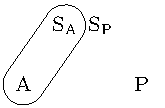
\includegraphics[\width=\linewidth]{figures/alignment}
Participant indexing on verbs thus displays split-intransitive alignment: active verbs index transitive and intransitive subjects identically while distinguishing objects (\ref{ex:alignment1}, \ref{ex:alignment2}). Stative verbs do not index their invariably intransitive subject like active verbs do (\ref{ex:alignment3}), nor do their suffixes overlap with undergoer marking on transitive verbs (\ref{ex:alignment1}). An illustration is given in \Cref{fig:verb_alignment}.

\is{Alignment}
\begin{figure}
\begin{tikzpicture}
	\topnode{}
	\topleftnode[sa]{\gl{S\textsubscript{A}}}
	\toprightnode[sp]{\gl{S\textsubscript{P}}}
	\leftnode[a]{\gl{a}}
	\rightnode[p]{\gl{p}}
	\draw \convexpath{11.2pt}{a,sa};
	\draw (p) circle (11.2pt);
\end{tikzpicture}
% % 		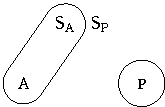
\includegraphics[width=0.3\linewidth]{figures/verb_alignment}
\caption{Verbal alignment}
\label{fig:verb_alignment}
\end{figure}


	\ea 
\label{ex:alignment1}
	\gll e=xhwii-ko\\
	 1\gl{sg}=bite-2\gl{sg}.\gl{obj} \\
	\glt \qu{I bite you.}
	\z
	
	
	\ea\label{ex:alignment2}
	\gll e=thana\\
	 1\gl{sg}=wander\\
	\glt \qu{I wander around.}
	\z
	
	
	\ea\label{ex:alignment3}
	\gll sinu-go\\
	 suffer-2\gl{sg}\\
	\glt \qu{You are ill, you suffer.}
	\z
	
	
	\ea\label{ex:WCstat_inan}
	\gll sinu (i=xh-ong)\\
	 suffer (\gl{def}.\gl{sg}=leg-1\gl{sg}.\gl{poss})\\
	\glt \qu{(My leg) hurts.}
	\z

The main types of verbs are the following.
\begin{enumerate}
	\item \emph{active transitive}: The subject marker precedes the verb (except in the imperative), and the verb takes an argument (see \sectref{ssec:TransV}); \textit{{e=xale-ke/ko}} \qu{I see it\slash you}.
	
	\item \emph{active intransitive}: The subject marker precedes the verb, the verb does not take an argument. \textit{{E=moo}} \qu{I stay}, \textit{a=yajen} \qu{it shakes, trembles}, \textit{a=temineen} \qu{it floats}. The productive transitive suffix \textit{-ke} and the older \textit{-i} can often be added to derive a transitive form (see \sectref{ssec:ke_i}).
	
	\item \emph{stative}: stative verbs are directly followed by their subject marker. The latter are bound to the verb stem and cannot choose their host, which is why I analyze them as suffixes rather than clitics; \textbf{\textit{me-o}} \qu{I die}. While the proclitic subject markers of active verbs are obligatory for all subjects, the stative subject markers are only obligatory for human arguments. They are almost, but not completely, identical to the object markers found on transitive active verbs with animate objects that are not expressed as noun phrases (see \Cref{tab:markers}). Stative verbs cover a few semantically defined, closed groups of words.
	\begin{itemize}
	\sloppy
		\item numerals (\textit{see-a} \qu{be.one-3\gl{sg}}, \textit{thaloo-lu} \qu{be.two-3\gl{du}}, \textit{thien-le} \qu{be.three-3\gl{sg}})
		\item semantically ``patientive" verbs like \textit{sinu-ong} \qu{suffer-1\gl{sg}} \qu{I am sick/ I suffer}, \textit{xhwiiti-o koo-n} \qu{long.after-1\gl{sg} \gl{obl}-3\gl{sg}} \qu{I miss it}
		%\item demonstratives \textit{ehni-o} \qu{this is me, here I am}
		\item \textit{heeve-o/-go/-a} \qu{where-1\gl{sg}/-2\gl{sg}/-3\gl{sg}} \qu{where am I/are you/is s/he}
		\item verbs with ``adjectival meanings" like \textit{vun-go} \qu{blue/green-2\gl{sg}} \qu{you are blue/green}, \textit{xhopwe-} \qu{(be) grow(n)}, \textit{mapehno-le} \qu{they are few}
	\end{itemize}
	\item There is also a group of verbs that cannot occur alone. They are not transitive, nor can they take subject markers, and they occur before or after another, independent, verb. These bound roots (called roots because they take no morphology on their own) are further described in \sectref{ssec:MannerV}.%, in things like \textit{vwa-thuan-ke} \qu{do-well-\textsc{tr}} looks like a compound.
\end{enumerate}

\section{Adverbs}
\is{Adverbs}
\label{sec:WCAdverbs}
Vamale possesses a small class of adverbs. They occur at the end of a clause or phrase, are frequently fronted without a phrase (\ref{ex:Adv}), take neither articles nor any kind of possessive or inflectional morphology, and are, if at all, modified by the intensifiers described in \sectref{sec:WCIntensifiers}, \textit{juu} \qu{real, really, very}. As they modify verb, noun, and prepositional phrases, and as they can be fronted alone, this analysis considers them to be adjuncts. Most members are transparently derived from nouns or prepositional phrases. See \sectref{sec:Adv} for examples of their interaction with verb and noun phrases. Example (\ref{ex:Adv}) features two cases of fronted adverbs,  (\ref{ex:Adv2}) shows an adverb at the end of a verb phrase, and (\ref{ex:Adv3}) shows an adverb after noun phrase.\largerpage[-2]

\ea
\label{ex:Adv}
(Adverbs are in bold, brackets show phrases, the comma separates two clauses)\\
\gll ka {\ob}jethro{\cb} \textbf{canbwen} man \textbf{bwethalo} {\ob}le=cuut cahni ka ni=bee-m-ca{\cb}, \textbf{cahni} {\ob}ca-n xhoogo{\cb}\\
 \gl{cnj} J. yesterday \gl{com} two.days.ago 3\gl{pl}=stand here \gl{sbj} \gl{def}.\gl{pl}=peer-2\gl{sg}.\gl{poss}-\gl{prox} here in-\gl{nspec} home\\
\glt \qu{And Jethro, yesterday and the day before your relatives stood here, here at home.} {[CP1:29]}
\z


\ea\label{ex:Adv2}
\gll e=ha-mwa \textbf{canbwen}\\
 1\gl{sg}=go-\gl{rep} yesterday\\
\glt \qu{I went back yesterday.} {[B2:134]}
\z


\ea\label{ex:Adv3}
\gll na i=vaaya-n xayu \textbf{habu} ka\\
 \gl{dem} \gl{def}.\gl{sg}=work-\gl{poss} man before \gl{disc}\\
\glt \qu{This was a man's work back then, like.} {[AG1:160]}\\
\z

\subsection{Temporal adverbs}
\label{ssec:TempAdv}

Temporal adverbs are a closed class of words that can occur in a fronted position (\ref{ex:tempadv}). They cannot take articles. Temporal adverbs were almost all derived from nominals, compare \textit{bwaabwen} \qu{morning} is related to the adverb \textit{bwaabwen-an} \qu{in the morning after}. Members include \textit{ca-n-bwen} \qu{yesterday (lit. \qu{in-\gl{nspec}-night})}, \textit{naen} \qu{today/now}, \textit{xahmaen} \qu{tomorrow}\footnote{Proto (Southern) Oceanic *marani \parencite[314]{lynch_efate-erromango_2004}.}, \textit{jimin} \qu{late at night (after having fallen asleep)}, \textit{bwethaloo} \qu{two days ago}, \textit{thaloobwen} \qu{overmorrow (lit. `two nights')}, \textit{daboo-n bwen} \qu{midnight (`lit. puddle/lake of the night')} %19-07-18, page 34)
\textit{hnyanan} \qu{constantly (lit. `its breath')}, \textit{mati} \qu{earlier}, \textit{mu-bwen} \qu{early in the morning (lit. `little night')}, \textit{nyeet} \qu{when?}, \textit{ca-li-been} \qu{sometimes (lit. `among the others')}. 

\ea \label{ex:tempadv}
\gll na li=\textit{peintures} habu\\
 \gl{dem} \gl{def}.\gl{pl}=paint before\\
\glt \qu{It's the (style of) painting from the old days.} {[KG:21]}
\z

\subsection{Locative adverbs}
\label{ssec:WCLocAdv}
A closed class of words describes locations. They are mostly derived from movement verbs.\footnote{\textit{Patemwano} \qu{directly next to it}, \textit{ngangeno} \qu{close-by} in Pije \parencite[170]{haudricourt_dictionnaire_1982} and \textit{puput} \qu{behind (a building or a sizeable entity)} can be used in the same slots but do not possess the morphological combinatorics shown in \Cref{tab:LocAdv}.} They do not bear articles, can be fronted alone (\ref{ex:front_xahut}), and can modify verbs (\ref{ex:xahut1}) as well as nouns (\ref{ex:LocAdvPred}). Locative adverbs can be predicates, see (\ref{ex:LocAdvPred}). Contrary to relational nouns (\sectref{ssec:WCPrepoNouns}), locative adverbs do not form possessive relations with nouns, nor do they take generic \textit{-n}. \Cref{tab:LocAdv} shows a summary of the forms. For a more thorough account of space (see \sectref{ssec:spat_adv}).
%members: (\textit{xahan}, \textit{xahut}, \textit{xada}, \textit{xahnuut}, \textit{xahnuda}, \textit{nya-xahan} etc, possibly \textit{patemwano}

\begin{table}
	\caption{Locative adverbs}
	\fittable{\begin{tabular}{lllll}
		\lsptoprule
	                &      & Simple & \\
		Axis		& Verb & location & Close-by& Further away\\
		\midrule
		same-level& \textit{han}& \textit{xa-han}& \textit{nya-xa-han} & \textit{nya-an xa-han}\\
		downward & \textit{hut}& \textit{xa-hut} & \textit{nya-xa-hut} & \textit{nya-ut xa-hut}\\
		upward & \textit{ta} &	\textit{xa-da} & \textit{nya-xa-da} & \textit{nya-da xa-da} \\
		downstream & \textit{hnuut}& \textit{xa-hnuut}& \textit{nya-xa-hnuut} & \textit{nya-hnut xa-hnuut}\\
		upstream & \textit{hnuuda} & \textit{xa-hnuuda} & \textit{nya-xa-hnuuda}& \textit{nya-hnuda xa-hnuuda}\\
		\lspbottomrule
	\end{tabular}}
\label{tab:LocAdv}
\end{table}


\ea\label{ex:xahut1}
\gll go=moo xahut, go=xahut, go=hut xahut\\
 2\gl{sg}=stay below 2\gl{sg}=below 2\gl{sg}=go.down below\\
\glt \qu{You live down there, you're down there, you go down there.}
\z


\ea\label{ex:front_xahut}
\gll xahut, go=majit mati\\
 below 2\gl{sg}=rest earlier\\
\glt \qu{Down there, you were sleeping earlier.}
\z


\ea\label{ex:LocAdvPred}
\gll i=apuli (a=) xahut\\
 \gl{def}.\gl{sg}=man (3\gl{sg}=) below\\
\glt \qu{The man is down there.}
\z

\subsection{\textit{hman} \qu{also}}
\textit{hman} \qu{also} modifies verbs (\ref{ex:hmanV}), nouns (\ref{ex:hman}), and adverbs. Contrary to temporal and locative adverbs, \textit{hman} always comes after the modified word and cannot be fronted on its own. Similarly to \textit{mwa} (\sectref{sec:mwa}), \textit{hman} is used as a discourse marker as well, with a meaning of \qu{however} (\ref{ex:hmanDisc}).

\ea\label{ex:hmanV}
\gll tha gau=han tha gau tha gase=bo \textit{arriver} hman\\
 \gl{ass} 2\gl{du}=go \gl{ass} 2\gl{du} \gl{ass} 1\gl{pl}.\gl{incl}=\gl{irr} arrive also\\
\glt \qu{You go (despite the height of the steel beam), you two, we'll get (to the other side), too.} {[KG:9]}
\z

\ea\label{ex:hman}
\gll li=meeka i=\ldots  li=nyan-mwa ca-n {hman}\\
 \gl{def}.\gl{pl}=all \gl{def}.\gl{sg}=\ldots \gl{def}.\gl{pl}=inside-house in-\gl{ana} also\\
\glt \qu{All the rooms in the house as well.} {[KG: 30-1]}
\z

\ea\label{ex:hmanDisc}
\gll thake yavo kavi tha cipa xhwii hman\\
 throw fishing.line but \gl{ass} \gl{neg} bite also\\
\glt \qu{...threw out the fishing line but it didn't bite though.} {[GP:73]}
\z

\section{Complementizer \textit{hapi}}
\is{Subordination!Complementation}
Clauses that are complement to verbs of cognition (\ref{ex:hapi2}), opinion, and perception (\ref{ex:hapi3}), are introduced by the subordinator \textit{hapi}. Considering \textcite{lynch_oceanic_2002}'s observation that Oceanic languages tend to use a form related or identical to the word \qu{to say} to introduce complement clauses \parencite[53]{lynch_oceanic_2002}, that Voh-Koné languages changed \textit{p-} $\rightarrow$ \textit{v-}, and that Hienghène languages have \textit{peei} \qu{to say}, \qu{\gl{comp}} \parencite[260]{haudricourt_dictionnaire_1982}, postulating \textit{a=vii} \qu{s/he says} as the origin of \textit{hapi} seems plausible.


\ea\label{ex:hapi2}
\gll e=caihna-n hapi tha hmwaana\\
 1\gl{sg}=know-\gl{nspec} \gl{comp} \gl{ass} thus\\
\glt \qu{I know that it's like that.}
\z


\ea\label{ex:hapi3}
\gll sahnaang-eong hapi tha hmwaana\\
 not.understand-1\gl{sg} \gl{comp} \gl{ass} thus\\
\glt \qu{I'm not sure/I doubt that it's like that.}
\z

\section{Conjunctions}
\label{sec:Conj}
Vamale distinguishes two groups of conjunctions: those that link noun phrases, and those that link verb phrases as well as clauses. Clauses are defined by the presence of a predicate, which is in most cases a verb phrase. This book calls the conjunctions linking these ``verbal", to distinguish them from nominal ones.   

\subsection{Nominal conjunctions}
\label{ssec:NomConj}

Nominal conjunctions connect noun (phrases) and form a new constituent containing the connected noun phrases and the conjunction. Members include \textit{ma} `and\slash with' (\ref{ex:maconj}), \textit{ka} `on the other hand' (\ref{ex:kaconj}), \textit{hai} \textasciitilde \textit{a} \qu{or} (\ref{ex:haiconj1}) with its derivative \textit{hai...hai} \qu{either...or} (\ref{ex:haiconj}),  \textit{moko} \qu{more than}. \textit{Moko} may be complex and composed of \textit{moo} \qu{rest, reside} and \textit{ko} \qu{on} (\sectref{sec:Comp}). It has no Hienghène cognate. The other Voh-Koné varieties share the form, however. \citet[215]{rivierre_bwatoo_2006} suggest a makeup of \textit{mo} \qu{from}, as in \textit{e ha-me \textbf{mo} Tuo} \qu{I come \textbf{from} Touho}, and \textit{ko} \qu{on}. 


\ea\label{ex:maconj}
\gll i=wabatan ma i=xat\\
 \gl{def}.\gl{sg}=north.wind and \gl{def}.\gl{sg}=sun\\
\glt `the north wind and the sun'
\z


\ea\label{ex:kaconj}
\gll i=wabatan ka i=xat\\
 \gl{def}.\gl{sg}=north.wind and \gl{def}.\gl{sg}=sun\\
\glt `the north wind, and (on the other hand) the sun'
\z


\ea\label{ex:haiconj1}
\gll i=wabatan hai i=xat\\
 \gl{def}.\gl{sg}=north.wind or \gl{def}.\gl{sg}=sun\\
\glt`the north wind or the sun'
\z


\ea\label{ex:haiconj}
\gll hai i=wabatan hai i=xat\\
 or \gl{def}.\gl{sg}=north.wind or \gl{def}.\gl{sg}=sun\\
\glt \qu{either the north wind or the sun}
\z

\subsection{Verbal conjunctions}
\label{ssec:VerbConj}

\is{Coordination!Verbal conjunctions}
The set of verbal conjunctions is small and closed, and groups together some morphemes which only occur in this set, like \textit{kavi} \qu{but}, with words also present in other distributional classes. The meaning distinctions between \textit{kavi} \qu{but (introducing something in contrast with the former element)}, \textit{ko} \qu{but [introducing something unexpected)}, and \textit{ma} \qu{but (relaying something related but different)} are fine and depend on the context. Members include \textit{ka} `and' (\ref{ex:kaVC}), \textit{kavi} `but' (\ref{ex:kaviVC}), \textit{ma} `and, but' (\ref{ex:maVC}), \textit{hai} \goodtilde \textit{a} `or' (\ref{ex:haiVC}), \textit{ko} \qu{but}, \qu{because}, \textit{kona} \qu{furthermore}. 


\ea\label{ex:kaVC}
\gll le=hame ka le=siwa=mwa\\
 3\gl{pl}=come and 3\gl{pl}=return=\gl{rep}\\
\glt `They came and they left again.'
\z


\ea\label{ex:kaviVC}
\gll le=hame kavi le=siwa-mwa\\
 3\gl{pl}=come but 3\gl{pl}=return-\gl{rep}\\
\glt `They came but they left again.'
\z


\ea\label{ex:maVC}
\gll le=ha-me ma le=siwa-mwa\\
 3\gl{pl}=go-\gl{dir.cp} and 3\gl{pl}=return-\gl{rep}\\
\glt `They come and/in order to go.'
\z


\ea\label{ex:haiVC}
\gll le=ha-me hai le=siwa=mwa\\
 3\gl{pl}=go-\gl{dir.cp} or 3\gl{pl}=return=\gl{rep}\\
\glt `They come or they go.'
\z

\textit{Ka} is also used colloquially after a clause to ask for confirmation (\ref{ex:kaDisc}) (see \sectref{discourse ka}).

\ea \label{ex:kaDisc}
\gll i=apuli a=xahan ka?\\
 \gl{def}.\gl{sg}=person \gl{rel}=over.there \gl{disc}\\
\glt \qu{The guy over there, like?}
\z

%\subsubsection{Numeral coordinators \textit{na-bwa}, \textit{ko}}
\is{Coordination!Numeral coordinators}
Numbers are verbal, and \textit{(na)-bwa} \qu{plus} (possibly from \gl{dem}-\qu{head}, \ref{ex:nabwa}), and \textit{ko} \qu{times} (probably from \textit{ko} \qu{on}) are used to construct complex numbers (\ref{ex:nabwako}). 


\ea\label{ex:nabwa}
(nim a-bwa se)\\
\gll nim na-bwa se\\
 5 plus 1\\
\glt \qu{6}
\z


\ea\label{ex:nabwako}
\gll nim na-bwa se ko apuli nabwa nim na-bwa se\\
  5 plus 1 times man/20 plus 5 plus 1\\
\glt \qu{126}
\z

\section{Subordinators}

Vamale subordinators introduce a subordinated clause. They precede all other elements of said clause, and cannot occur without the clause, moving with it if fronted, see examples (\ref{ex:fronted}--\ref{ex:frontedend}). All those ending on -\textit{a} assimilate to following \textit{e=} \qu{1\gl{sg}}. They are proclitics.
Members include \textit{cala} `when' \textit{cama} `if', \textit{ma} `as\slash in order to', \textit{ko} `because', \textit{ko-ma} `so that',  \textit{ecupwa}  \qu{until}.\footnote{Possibly from \textit{e-cuut-pwa} \qu{\gl{refl}-stand-on}.}

\ea \label{ex:fronted}
\gll cel=e=hame go=pa yahan\\
 when=1\gl{sg}=come 2\gl{sg}=\gl{prf} leave\\
\glt `When I came, you had already left.'
\z


\ea
\gll cala go=hame e=pa yahan\\
 when 2\gl{sg}=come 1\gl{sg}=\gl{prf} leave\\
\glt `When you came, I had already left.'
\z


\ea
\gll cem=e hame go=pa yahan\\
 if/when=1\gl{sg} come 2\gl{sg}=\gl{prf} leave\\
\glt `If I come, you will already have left.' \\'Whenever I come, you already have left.'
\z


\ea
\gll cama go=hame e=pa yahan\\
 if/when 2\gl{sg}=come 1\gl{sg}=\gl{prf} leave\\
\glt `If you come, I will already have left.' \\ `Whenever you come, I already have left'
\z


\ea
\gll m=e hame go=pa yahan\\
 as=1\gl{sg} come 2\gl{sg}=\gl{prf} leave\\
\glt `As I come, you've already left.'
\z


\ea \label{ex:frontedend}
\gll ma le=fe, le=mu=xaahni\\
 as 3\gl{sg}=take, 3\gl{pl}=\gl{freq}=check\\
\glt \qu{When they take it, they check it.}
\z

Non-fronted examples, illustrated in (\ref{ex:non-fronted}), are the norm.

\ea \label{ex:non-fronted}
\gll tha=abe=saavi cama=abe icu-koo-n ko-n \textit{marché}\\
 \gl{ass}=1\gl{pl}.\gl{excl}=dig.up \gl{subr}=1\gl{pl}.\gl{excl} trade-\gl{obl}-\gl{ana} on-\gl{nspec} market\\
\glt `We dig (them) up when we sell them on the market.' {[AG1:22]}
\z


\ea
\gll le=thêên cala le=siwa-mwa\\
 3\gl{pl}=run when.\gl{real} 3\gl{pl}=return-\gl{rep}\\
\glt \qu{They ran when they went back.}
\z

\ea
\gll le=thêên ma le=yahan\\
  3\gl{pl}=run when.\gl{irr}/if 3\gl{pl}=leave\\
\glt `(Usually) they run when they leave.' / `They would run if they left.'
\z


\ea
\gll e=ha-me ma go=bwa=yahan\\
 1\gl{sg}=go-\gl{dir.cp} \gl{subr} 2\gl{sg}=\gl{ipfv}=leave\\
\glt `I come as as you leave.' / `I come if you leave.' / `I come so that you leave.'
%\a
%
%\gll le=ɣahni ma le=fe
%
% 3\gl{pl}=check in.order.to 3\gl{pl}=take
%
%\glt \qu{they're checking to take}
%
%
\z




\section{Negation markers}
\is{Negation}

The negation markers \textit{cipa} \qu{\gl{neg}} and \textit{cipii} \qu{\gl{proh}} share their scope over the entire following clause and their left-most position. The negation markers are not identical in their distribution and could, strictly speaking, be classified into two separate classes. Contrary to \textit{cipa} \qu{\gl{neg}} (\ref{ex:thacipa}), \textit{cipii} \qu{\gl{proh}} cannot take assertive \textit{tha}, nor \textit{na} \qu{\gl{foc}}. Furthermore, \textit{cipii} often omits the subject marker, which \textit{cipa} cannot do (\ref{ex:cipi}). This grammar will treat \textit{cipa} as a proclitic, because it integrates into the following verb phrase's stress structure, and assimilates phonologically to it as well (\ref{ex:cipa}).
%

	
	\ea\label{ex:thacipa}
	\gll (tha) cipa {\ob}go=bwaa=majit{\cb}?\\
	 (\gl{ass}) \gl{neg} 2\gl{sg}=\gl{ipfv}=sleep\\
	\glt \qu{Aren't you still asleep?}
	\z
	
	
	\ea\label{ex:cipa}
	[ˌci.pe.ˈmãn.ɟit]\\
	\gll cipa= e= majit\\
	 \gl{neg} 1\gl{sg}= sleep\\
	\glt \qu{I don't sleep.}
	\z
	
\ea \label{ex:cipi}
\gll cipii xaloo koo-ng hmwaahni (ka go)! \\
 \gl{proh} gaze \gl{obl}-1\gl{sg}.\gl{poss} thus \gl{sbj} 2\gl{sg}\\
\glt \qu{Don't look at me like that!}
\z

\section{Assertive \textit{tha}}
\label{sec:WCAssertive}
\is{Assertive \textit{tha}}

The assertive marker \textit{tha} is a proclitic that docks onto the predicates of non-imperative clauses, on the left-most position (\ref{ex:tha1}). \textit{Tha} assimilates to \textit{e=} \qu{1\gl{sg}}, like \textit{cipa} \qu{\gl{neg}} (\ref{ex:tha2}). %unlike \textit{na} \qu{\gl{dem}}, pro-clitic to predicates.



\begin{exe}[(999)]
\ex \label{ex:tha1}
\gll \textit{au lieu} ma tha bwa xhavwale i=\textit{copain}-ea vukin tha=a bo \textit{guide}-ea\\
 instead \gl{subr} \gl{ass} \gl{ipfv} wait \gl{def}.\gl{sg}=friend-3\gl{sg}.\gl{poss} reason \gl{ass}=3\gl{sg} \gl{irr} guide-3\gl{sg}.\gl{poss}\\
\glt \qu{Instead of waiting for his friend, because he would be his guide!} {[KG:497]}
\end{exe}


\ea\label{ex:tha2}
\gll cala th=e vwa-tau \\
 when \gl{ass}=1\gl{sg} do-impact\\
\glt \qu{when I fish} {[B3:3]}
\z

\section{Intensifiers}
\label{sec:WCIntensifiers}
\is{Intensifiers}

The two intensifiers \textit{juu} \qu{real, very} and \textit{vaa} \qu{(too) much} (most often preceded by \textit{juu}, but see \ref{ex:vaa}) cannot stand alone, are semantically vague (see \Cref{tab:juu}), and attach to the head of a phrase (be that a noun, an adverb, or anything else, \ref{ex:juu}) as closely as possible. Given that they can be stressed, they are analyzed as particles, though ``anti-clitic" may be a better term considering the fact that they syntactically depend on a host that can be nominal, verbal, or adverbial in nature. \textit{Juu} is also associated to \textit{bwa} \qu{\gl{ipfv}}, as described in \sectref{ssec:bwa_ju}.


\ea\label{ex:juu}
\gll a=juu hnyimake ka i=juu apuli, juu ca-n-bwen\\
 3\gl{sg}=very think \gl{sbj} \gl{def}.\gl{sg}=real person real in-\gl{nspec}-night\\
\glt `He thought hard, the real man, just yesterday.'
\z


\ea\label{ex:vaa}
\gll ma go=hmwaani vwasoon, ma go=hmwaani vaa...\\
 \gl{cond} 2\gl{sg}=like.this impossible \gl{cond} 2\gl{sg}=like.this too.much\\
\glt \qu{If you do it like this, it's impossible, and if you do it like this, it's too...} {[KG:140]}
%\a
%
%\gll na li=a le=ɣaleke
%
% DEM.PRED SPEC.PL REL 3PL=see
%
%\glt `It is they who watched.'
%
%
\z


\begin{table}
	\caption{Meanings of compounds with \textit{juu}}
	\begin{tabular}{lll}
	\lsptoprule
		Form & \multicolumn{2}{c}{Translation of}\\\cmidrule(lr){2-3}
		     & the 2nd morpheme & the whole\\
	\midrule
		\textit{juu han} & walk & \qu{walk barefoot}\\
		\textit{juu aman} & thing & \qu{important (adverb)}\\
		\textit{juu we} & water & \qu{drinking water} \\
		\textit{juu toot} & grass & \qu{thatching grass}\\
		\textit{juu o} & bamboo & \qu{building bamboo}\\
		\textit{juu mwa} & house & \qu{trad. house}\\
		\textit{juu mani} & bird & \qu{{notou} {[ducula goliath]}}\\
		\textit{juu apuli} & person & \qu{Kanak}\\
		\textit{juujuu} & & \qu{truth}\\
	\lspbottomrule
	\end{tabular}
\label{tab:juu}
\end{table}

The particle \textit{vaa}, depending on the word it modifies, means \qu{much (uncountable)} with non-human nouns (\ref{ex:vaa1}), %meaning \qu{many} for ants, in contrast to \textit{hmain}, \qu{many} for humans.
 intensifies the following verb, e.g. \textit{vaa thêên} \qu{strongly run}\slash\qu{run fast}, and in combination with \textit{ju} \qu{real, true}, it means \qu{too much}, as in (\ref{ex:vaa2}). 


\ea\label{ex:vaa1}
\gll e-vaa nya-da xa-da\\
 \gl{mid}-\gl{ints} towards-up.there \gl{loc}.\gl{adv}-up \\
\glt \qu{There are many (feral pigs) up there.} {[J3 16.1]}
\z


\ea \label{ex:vaa2}
\gll juu va vwasoon ma gase=vwa li=vaaya-n li=xhaohmu\\
 real much difficult \gl{comp} 1\gl{pl}.\gl{incl}=do \gl{def}.\gl{pl}=work-\gl{poss} \gl{def}.\gl{pl}=elder\\
\glt \qu{It's too hard for us to do the work of the elders.} {[KP:98]}
\z



\section{Repetitive \textit{mwa}}
\label{sec:WCRepetitive}
\is{Repetitive \textit{mwa}}

This class only has one member. \textit{Mwa} has rather different, related meanings, depending on the context. \textit{Mwa} can have the repetitive meaning \qu{again} (\ref{ex:mwa_even}), the restitutive \qu{back}, as well as \qu{also}, \qu{even}, \qu{on top of that}, or mark the preceding phrase as focused (see \sectref{sec:mwa} for a discussion). The deictic use of \textit{mwa} \qu{now} (\ref{ex:mwa}), seems to mostly anchor the listener's attention, similarly to \textit{mwa} \qu{even}, onto the noun phrase given, see (\ref{ex:mwa_now1a}). \textit{Mwa} is a particle that can dock onto any phrase preceding it (see \ref{ex:mwa_rep}).

\ea\label{ex:mwa_even}
\gll e=xaleke mwa\\
 1\gl{sg}=see \gl{rep}\\
\glt `I see again.', `I even see.'
\z

\ea
\label{ex:mwa_rep}
\gll e=vatipwe mwa nya-mwa si-m mwa i=mwani mwa\\
 1\gl{sg}=drop \gl{rep} give-\gl{rep} hand-2\gl{sg}.\gl{poss} \gl{rep} \gl{def}.\gl{sg}=money \gl{rep}\\
\glt \qu{I pass on to you too this money as well.}
\z


\ea\label{ex:mwa}
\gll hê na tha vwa li=wii-n. go le=vwa ibi-han li=nyamaan go tha le=ve-moo mwa, moo mwa. \\
 yes \gl{dem} \gl{ass} \gl{exist} \gl{def}.\gl{pl}=field-\gl{poss}.\gl{nspec} then 3\gl{pl}=do pinch-walk \gl{def}.\gl{pl}=eye then \gl{ass} 3\gl{pl}=\gl{mid}-stay \gl{rep} stay \gl{rep}\\
\glt \qu{Yes there were fields of it (macaranga vedeliana). And they'd go pinch the young sprouts. And those stay together now, stay.} {[KL:218-222]}
\z


\ea\label{ex:mwa_now1a}
\gll ya a=ja vwa \textbf{mwa} li=wee-n a=ta-\textbf{mwa} sibu li=sibu \textbf{mwa}. ja yabwat \textbf{mwa} sisuu \textbf{mwa}\\
 \gl{expl} 3\gl{sg}=\gl{prf} do \gl{rep} \gl{def}.\gl{pl}=water-\gl{poss}.\gl{nspec} 3\gl{sg}=go.up-\gl{rep} swell \gl{def}.\gl{pl}=swell \gl{rep} \gl{prf} dry \gl{rep} hard \gl{deict}\\
\glt \qu{And there's the sap that rises, swells, the swells there. It dries then, gets hard then.}
\z

In (\ref{ex:movV-mwa1}) and for all other movement verbs, as well as \textit{xhose} \qu{do again}, \textit{mwa} is analyzed as a suffix, i.e. as having fused with its host. First, \textit{mwa} assimilates to the root, which it does not do in other contexts.\footnote{\textit{Xhosepwa} suggests a dropped \textit{-t} or \textit{-p}. The Pije and Fwâi cognates \textit{khô-peei} \qu{?-say} \parencite[155]{haudricourt_dictionnaire_1982} could be a diachronic hint at a morphologically complex, old Vamale form.} Compare \textit{hut-mwa} $\rightarrow$ /hupʷa/ \qu{go back down}, to \textit{hut=mwa} \qu{go down again}.

%\begin{multicols}{2}
\ea \label{ex:movV-mwa1}
\gll go=ha-mwa-me\\
 2\gl{sg}=go=\gl{rep}=\gl{dir.cp}\\
\glt \qu{You return to me, you come back.}
\z


\ea
\gll go=ha-me mwa\\
 2\gl{sg}=go=\gl{dir.cp} \gl{rep}\\
\glt \qu{You come again.}
\z
%\end{multicols}

The particle also expresses repetition (\ref{ex:mwa_rep1a}), and deictically referring to something close spatially or recently mentioned (which is probably a derived meaning), as in (\ref{ex:mwa_rep1b}). See \sectref{sec:mwa} for a more detailed description. %Also means "even, on top of that". 


\ea\label{ex:mwa_rep1a}    
\gll e=tena mwa\textsuperscript{{\upshape REP}} i=hun-det\\
 1\gl{sg}=hear \gl{rep} \gl{def}.\gl{sg}=\gl{nmlz}-sound\\
\glt \qu{I hear the sound again.} {[JR:17]}
\z

\ea\label{ex:mwa_rep1b}
\gll xhose e=tena mwa\textsuperscript{{\upshape REP}} tha=a=bwa vwa det mwa\textsuperscript{{\upshape\gl{deict}}}\\
 again 1\gl{sg}-feel \gl{rep} \gl{ass}=3\gl{sg}=\gl{ipfv} do sound \gl{rep}\\
\glt \qu{Again I heard him make said (\textit{mwa}) noise.} {[JR:18]}
\z 


%intransitive und transitive stämme in vamale müssen nicht postuliert werden, bzw. kein unterschied zu intransitiven und transitiven wurzeln

\section{Interjections}
\is{Interjections}
Interjections do not integrate into clauses or phrases, and though at least \textit{hê} \qu{yes} can be derived to \textit{hêêke} \qu{to assent, to say yes}, and \textit{cika} \qu{\gl{neg}.\gl{exist}} is a commonly used impersonal verb, exclamations form a group through their uniquely individualistic behavior.
Members include \textit{ya} \qu{voilà, the result is there}, \textit{ûhû}\slash\textit{cika} \qu{no}, \textit{hat} \qu{strong negation}, \textit{hai} \qu{oh! (surprise, discovery)} and \textit{hê}\slash\textit{helong} \qu{yes}, as well as a growing class of swearwords. 

\section{Quantifiers}
\is{Noun phrase!Quantifiers}
Quantifiers are a tiny group of particles that are not inflected, directly preceding an (article) noun construction: \textit{mu} \qu{little}, \textit{jaa} \qu{many} (\ref{ex:jaa}), and \textit{ju-vaa} \qu{too much}, which is also attested as an intensifier in verb phrases (\ref{ex:juva}). Quantifiers denote number and are described in \sectref{ssec:Quant}. Other words have similar meanings, but are verbs, like \textit{hmai-} \qu{many}. One quantifier similarly integrates the noun phrase, but bears possessive suffixes: \textit{meeka-n} \qu{all}.



	\ea\label{ex:jaa}
	\gll ja apuli canbwen\\
	 many people yesterday\\
	\glt \qu{(there were) more people yesterday (than now)} {[B2 31.1]}
\z	
	
	\ea\label{ex:juva}
	\gll ju-vaa apuli\\
	 too.much person\\
	\glt \qu{too many people} {[B2:32]}
	\z
	


%\section{Conclusion}
%Does it even need to have a conclusion?
%\begin{quote}
%	Vamale wordos:\\
%	They differ like spring flowers\\
%	Behold the garden.\\
%\end{quote}
%\begin{table}
%\begin{tabular}{p{3cm}|c|c|c|c|c|c}
%takes / appears in & nouns & \multicolumn{2}{c}{verbs} & adverbs & \\
%\midrule
%&& active& stative&&&\\
%\midrule
%Articles & x &&&&&\\
%Possessive suffixes& x &&&& &\\
%S/A- markers and -O markers&  & x&&&&\\
%-S markers& && x&&&\\
%in NP& x &&& x& &\\
%in VP&& x& x&& x&\\
%\end{tabular}
%\caption{Word classes}
%\label{tab:WordClasses}
%\end{table}
